\chapter{Successful architectures}


\section{Preliminaries}

\begin{description}
    \item[Stem layer] \marginnote{Stem layer}
        First convolutional layer(s) of a CNN that aims to reduce the spatial size of the activations for memory and computational purposes
        but also to rapidly increase the receptive field.

    \item[Model parallelism] \marginnote{Model parallelism}
        Train a model by splitting its weights on multiple computational units, each receiving the same data.

    \item[Data parallelism] \marginnote{Data parallelism}
        Train a model by distributing the data on multiple computational units, each with a copy of the weights of the model.

    \item[Overlapping pooling] \marginnote{Overlapping pooling}
        Pooling layer with kernel size and stride chosen in such a way that
        some pixels at a step have also been considered at the previous one (e.g. $3 \times 3$ kernel with stride $2$).

    \item[$1 \times 1$ convolution] \marginnote{$1 \times 1$ convolution}
        Convolution used to change the depth of the activation while maintaining its spatial dimension.
        It can be seen as a linear fully connected layer at each spatial dimension.

        \begin{figure}[H]
            \centering
            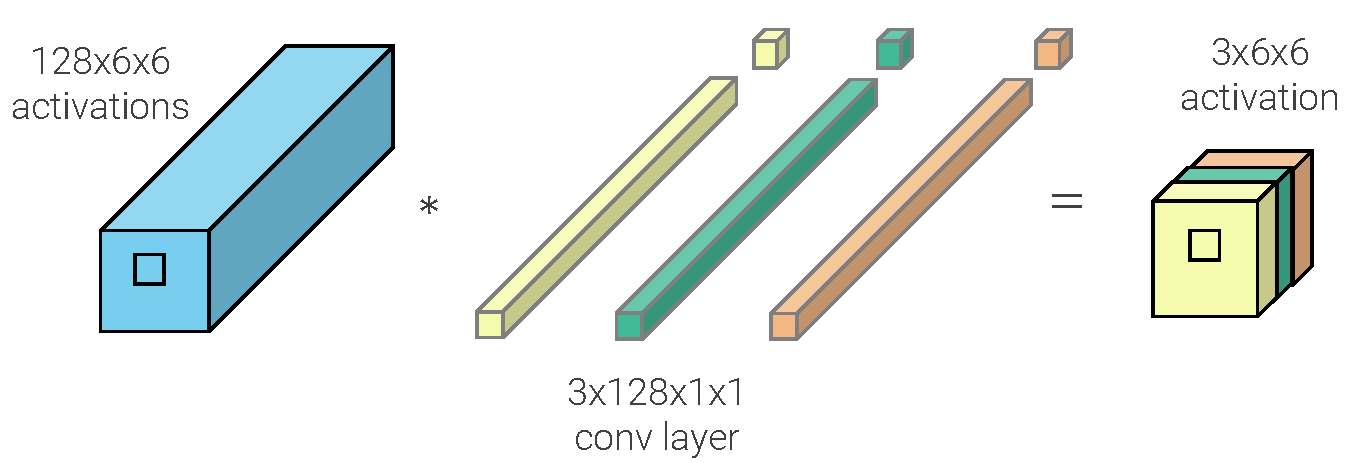
\includegraphics[width=0.55\linewidth]{./img/_1conv.pdf}
        \end{figure}

        \begin{remark}
            Stacking multiple $1 \times 1$ convolutions is equivalent to a multi-layer perceptron 
            (i.e. universal function approximator).
        \end{remark}

    \item[Parameters computation] \marginnote{Parameters computation}
        \phantom{}
        \begin{description}
            \item[Input layer]
                Given an input image of shape $W_\text{in} \times H_\text{in} \times C_\text{in}$,
                the number of activations in the input layer is given by:
                \[ \texttt{\#activations} = W_\text{in} \cdot H_\text{in} \cdot C_\text{in} \]

                % As data is processed in batches of size $B$, the actual number of activations is:
                % \[ \texttt{\#activations\_batch} = B \cdot \texttt{\#activations} \]

            \item[Convolutional layer]
                Given:
                \begin{itemize}
                    \item An input of shape $W_\text{in} \times H_\text{in} \times C_\text{in}$,
                    \item A kernel of shape $W_\text{K} \times H_\text{K}$ with padding $P$ and stride $S$,
                    \item A desired number of output channels $C_\text{out}$,
                \end{itemize}
                the number of parameters of a convolutional layer (see \Cref{sec:conv_layer}) is given by:
                \[ \texttt{\#params} = \big( (W_\text{K} \cdot H_\text{K} \cdot C_\text{in}) + 1 \big) \cdot C_\text{out} \]

                The output shape (see \Cref{sec:conv_layer}) and the number of activations is given by:
                \[  
                    \begin{gathered}
                        \texttt{activ\_w} = \left\lfloor \frac{W_\text{in} - W_\text{K} + 2P}{S} \right\rfloor + 1 \hspace{2em}
                        \texttt{activ\_h} = \left\lfloor \frac{H_\text{in} - H_\text{K} + 2P}{S} \right\rfloor + 1 \\
                        \texttt{\#activations} = \texttt{activ\_w} \cdot \texttt{activ\_h} \cdot C_\text{out}
                    \end{gathered}    
                \]

                The number of FLOPs for a single example of the batch is given by:
                \[ \texttt{FLOPs} = \texttt{\#activations} \cdot (W_\text{K} \cdot H_\text{K} \cdot C_\text{in}) \cdot 2 \]

            \item[Pooling layer]
                Given:
                \begin{itemize}
                    \item An input of shape $W_\text{in} \times H_\text{in} \times C_\text{in}$,
                    \item A kernel of shape $W_\text{K} \times H_\text{K}$ with padding $P$ and stride $S$,
                \end{itemize}
                the number of activations in a pooling layer is computed as above with $C_\text{in} = C_\text{out}$:
                \[ \texttt{\#activations} = \texttt{activ\_w} \cdot \texttt{activ\_h} \cdot C_\text{in} \]

                The number of FLOPs for a single example of the batch is given by:
                \[ \texttt{FLOPs} = \texttt{\#activations} \cdot (W_\text{K} \cdot H_\text{K}) \]

            \item[Fully-connected layer]
                Given:
                \begin{itemize}
                    \item An activation of shape $C_\text{in}$,
                    \item The number of neurons $C_\text{out} = \texttt{\#activations}$,
                \end{itemize}
                the number of parameters of a fully-connected layer is:
                \[ \texttt{\#params} = (C_\text{in} \cdot C_\text{out}) + C_\text{out}\]

                The number of FLOPs for a single example of the batch is given by:
                \[ \texttt{FLOPs} = 2 \cdot C_\text{in} \cdot C_\text{out} \]

            \item[Memory usage]
                Given:
                \begin{itemize}
                    \item The batch size $B$, 
                    \item The activation size $\texttt{\#activations}$, 
                    \item The number of parameters $\texttt{\#params}$, 
                \end{itemize}
                to estimate the memory consumption, the following have to be taken into account:
                \begin{itemize}
                    \item To compute the gradient of the loss, every intermediate activation for every example in the batch has to be stored.
                    \item For every parameter, we have to store its value and the gradient of the loss w.r.t. it.
                    \item Optimizers with momentum need to store more values per parameter.
                \end{itemize}

                It is therefore hard to estimate memory requirements. 
                A rule of thumb estimates a lower bound as twice the activation size and 3-4 times the number of parameters.
                Assuming that $\texttt{float32}$ (4 bytes) are used, memory consumption is computed as:
                \[
                    \begin{gathered}
                        \texttt{memory\_activ\_bytes} = 2 \cdot (B \cdot \texttt{\#activations} \cdot 4) \\
                        \texttt{memory\_params\_bytes} = 3 \cdot (\texttt{\#params} \cdot 4)
                    \end{gathered}  
                \]
        \end{description}
\end{description}


\section{LeNet-5}
\marginnote{LeNet-5}

LeNet-5 is one of the first convolutional neural networks.
The network has the following properties:
\begin{itemize}
    \item At each layer, the number of channels increases and the spatial dimension decreases.
    \item Convolutions have the following characteristics: $5 \times 5$ kernels, no padding and average pooling for down-sampling.
    \item \texttt{Sigmoid} and \texttt{tanh} activation functions are used, with carefully selected amplitudes (i.e. they are scaled).
    \item The last layers are fully connected with a radial basis function as the output activation.
    \item There are no residual connections and normalization layers.
\end{itemize}

\begin{figure}[H]
    \centering
    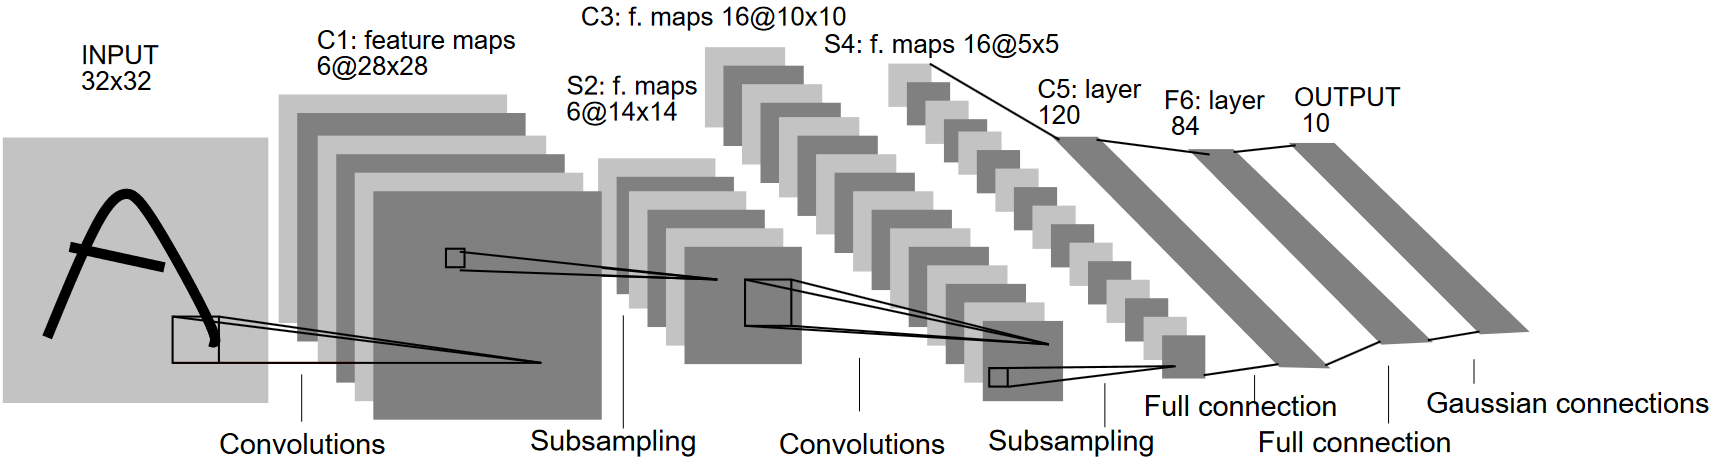
\includegraphics[width=0.7\linewidth]{./img/lenet5.png}
    \caption{LeNet-5 architecture}
\end{figure}



\section{AlexNet}
\marginnote{AlexNet}

AlexNet is the first CNN that broke the stagnation of the field.


\subsection{Architecture}

AlexNet is composed of:
\begin{itemize}
    \item 5 convolutional layers (convolution + \texttt{ReLU}, sometimes with max-pooling).
    \item 3 feed-forward layers.
\end{itemize}

\begin{remark}
    Some layers are normalized using local response normalization (more active neurons are enhanced and the others are inhibited).
\end{remark}

\begin{figure}[H]
    \centering
    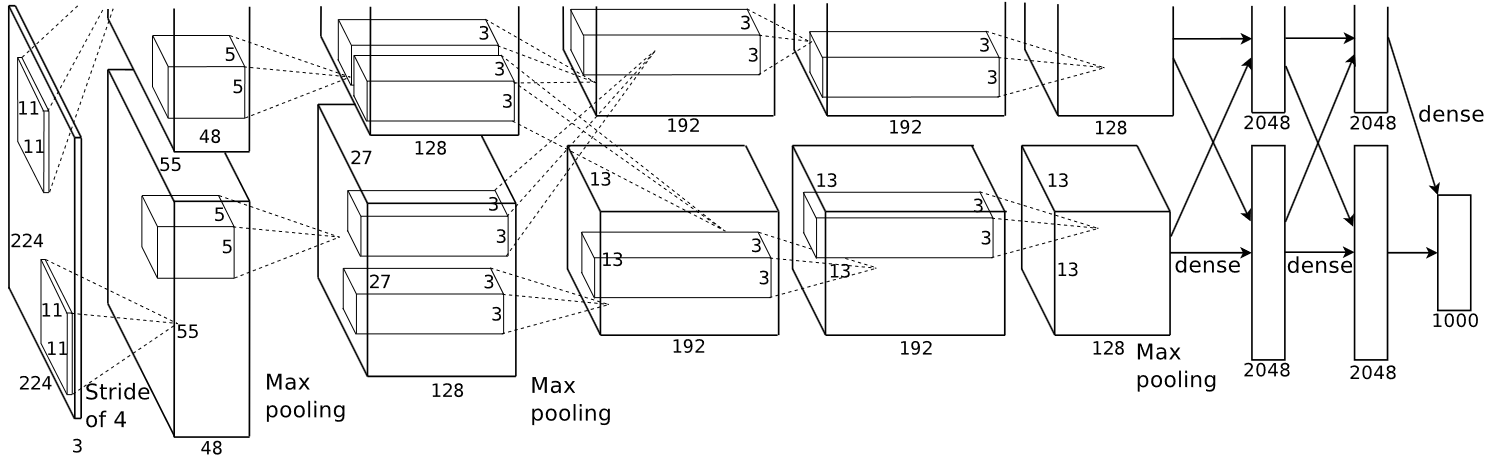
\includegraphics[width=0.75\linewidth]{./img/alexnet.png}
    \caption{AlexNet architecture}
\end{figure}


\subsection{Training}

The network was trained on ImageNet 1k (for the ILSVRC 2012) with a batch size of 128.
Due to GPU memory limitations, training was split into two parallel lines on two GPUs (model parallelism).

\begin{description}
    \item[Grouped convolution] \marginnote{Grouped convolution}
        A convolution is split into two sets of weights, each trained independently on a computational line.
        At some steps (e.g. \texttt{conv3}), the two GPUs are allowed to communicate.
        In this case, the result of the operation can be virtually seen as if it was done by a single computational unit (i.e. the operation is done on the full set of weights).
\end{description}

\begin{remark}
    At the time, training took 5-6 days on two NVIDIA GTX 580.
\end{remark}


\subsection{Properties}

AlexNet has the following trends:
\begin{itemize}
    \item The first convolutional layer is a stem layer.
    \item The majority of the parameters are in the fully connected layers (even though they have to process an activation of 4096 elements).
    \item The largest memory consumption for activations is at the first convolutional layer.
    \item The largest amount of FLOPs is required by the convolutional layers.
    \item The total number of parameters and activations at training time are relatively comparable.
    \item $2.2$ GFLOPs are required to process an image at training time.
\end{itemize}

\begin{table}[H]
    \centering
    \caption{Parameters of AlexNet (batch size of 128)}
    \scriptsize
    \begin{tabular}{cccccccccccc}
        \toprule
        \multirow{2}[20]{*}{\textbf{Layer}} 
            & \multicolumn{4}{c}{\textbf{Convolution}} 
            & \multicolumn{3}{c}{\textbf{Single activation}} 
            & \multicolumn{2}{c}{\textbf{Batch requirements}}
            & \multicolumn{2}{c}{\textbf{Parameters}} \\
        \cmidrule(lr){2-5} \cmidrule(lr){6-8} \cmidrule(lr){9-10} \cmidrule(lr){11-12}
            & \rot{\textbf{Channels}} & \rot{\textbf{H/W}} & \rot{\textbf{Stride}} & \rot{\textbf{Padding}} 
            & \rot{\textbf{H/W}} & \rot{\textbf{Channels}} & \rot{\texttt{\#activations}} 
            & \rot{\textbf{MFLOPs}} & \rot{\textbf{Activ. mem.}} & \rot{\textbf{Amount}} & \rot{\textbf{Memory}} \\
        \midrule
        \texttt{input}      & --          & --          & --          & --      & \num{227}   & \num{3}     & \num{154587}  & --              & \num{75.5} {\tiny MB}  & \num{0}                 & \num{0.0}              \\
        \cmidrule(lr){1-12}
        \texttt{conv1}      & \num{96}    & \num{11}    & \num{4}     & \num{0} & \num{55}    & \num{96}    & \num{290400}  & \num{26986.3}   & \num{283.6} {\tiny MB} & \num{35} {\tiny K}      & \num{0.4} {\tiny MB}   \\
        \texttt{pool1}      & \num{1}     & \num{3}     & \num{2}     & \num{0} & \num{27}    & \num{96}    & \num{69984}   & \num{80.6}      & \num{68.3} {\tiny MB}  & \num{0}                 & \num{0.0}              \\
        \cmidrule(lr){1-12}
        \texttt{conv2}      & \num{256}   & \num{5}     & \num{1}     & \num{2} & \num{27}    & \num{256}   & \num{186624}  & \num{114661.8}  & \num{182.3} {\tiny MB} & \num{615} {\tiny K}     & \num{7.0} {\tiny MB}   \\
        \texttt{pool2}      & \num{1}     & \num{3}     & \num{2}     & \num{0} & \num{13}    & \num{256}   & \num{43264}   & \num{49.8}      & \num{42.3} {\tiny MB}  & \num{0}                 & \num{0.0}              \\
        \cmidrule(lr){1-12}
        \texttt{conv3}      & \num{384}   & \num{3}     & \num{1}     & \num{1} & \num{13}    & \num{384}   & \num{64896}   & \num{38277.2}   & \num{63.4} {\tiny MB}  & \num{885} {\tiny K}     & \num{10.1} {\tiny MB}  \\
        \cmidrule(lr){1-12}
        \texttt{conv4}      & \num{384}   & \num{3}     & \num{1}     & \num{1} & \num{13}    & \num{384}   & \num{64896}   & \num{57415.8}   & \num{63.4} {\tiny MB}  & \num{1327} {\tiny K}    & \num{15.2} {\tiny MB}  \\
        \cmidrule(lr){1-12}
        \texttt{conv5}      & \num{256}   & \num{3}     & \num{1}     & \num{1} & \num{13}    & \num{256}   & \num{43264}   & \num{38277.2}   & \num{42.3} {\tiny MB}  & \num{885} {\tiny K}     & \num{10.1} {\tiny MB}  \\
        \texttt{pool3}      & \num{1}     & \num{3}     & \num{2}     & \num{0} & \num{6}     & \num{256}   & \num{9216}    & \num{10.6}      & \num{9.0} {\tiny MB}   & \num{0}                 & \num{0.0}              \\
        \cmidrule(lr){1-12}
        \texttt{flatten}    & \num{0}     & \num{0}     & \num{0}     & \num{0} & \num{1}     & \num{9216}  & \num{9216}    & \num{0.0}       & \num{0.0}              & \num{0}                 & \num{0.0}              \\
        \texttt{fc6}        & \num{4096}  & \num{1}     & \num{1}     & \num{0} & \num{1}     & \num{4096}  & \num{4096}    & \num{9663.7}    & \num{4.0} {\tiny MB}   & \num{37758} {\tiny K}   & \num{432.0} {\tiny MB} \\
        \texttt{fc7}        & \num{4096}  & \num{1}     & \num{1}     & \num{0} & \num{1}     & \num{4096}  & \num{4096}    & \num{4295.0}    & \num{4.0} {\tiny MB}   & \num{16781} {\tiny K}   & \num{192.0} {\tiny MB} \\
        \texttt{fc8}        & \num{1000}  & \num{1}     & \num{1}     & \num{0} & \num{1}     & \num{1000}  & \num{1000}    & \num{1048.6}    & \num{1.0} {\tiny MB}   & \num{4097} {\tiny K}    & \num{46.9} {\tiny MB}  \\
        \midrule
        &&&&&&& \textbf{Total} & \num{290851} & \num{1406} M{\tiny B} & \num{62378} {\tiny K} & \num{714} M{\tiny B} \\
        \bottomrule
    \end{tabular}
\end{table}



\section{ZFNet/Clarifai}
\marginnote{ZFNet/Clarifai}

The aggressive stem layer of AlexNet causes dead neurons that do not specialize in recognizing anything.

Ablation and visualization studies found out that the first stem layer works better if split into two layers
respectively with a $7 \times 7$ and $5 \times 5$ kernel, both with stride $2$.

\begin{figure}[H]
    \centering
    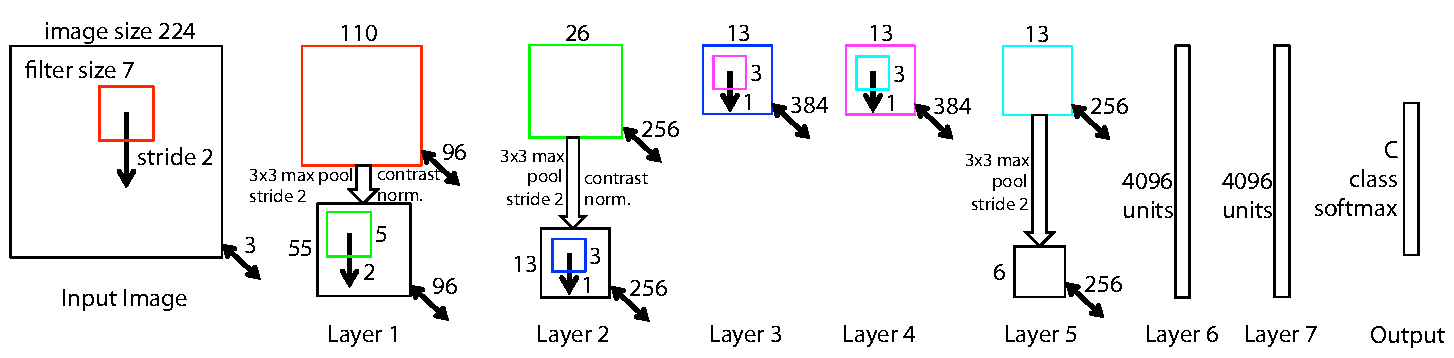
\includegraphics[width=0.8\linewidth]{./img/_zfnet.pdf}
    \caption{ZFNet architecture}
\end{figure}

\begin{figure}[H]
    \centering
    \begin{subfigure}{0.4\linewidth}
        \centering
        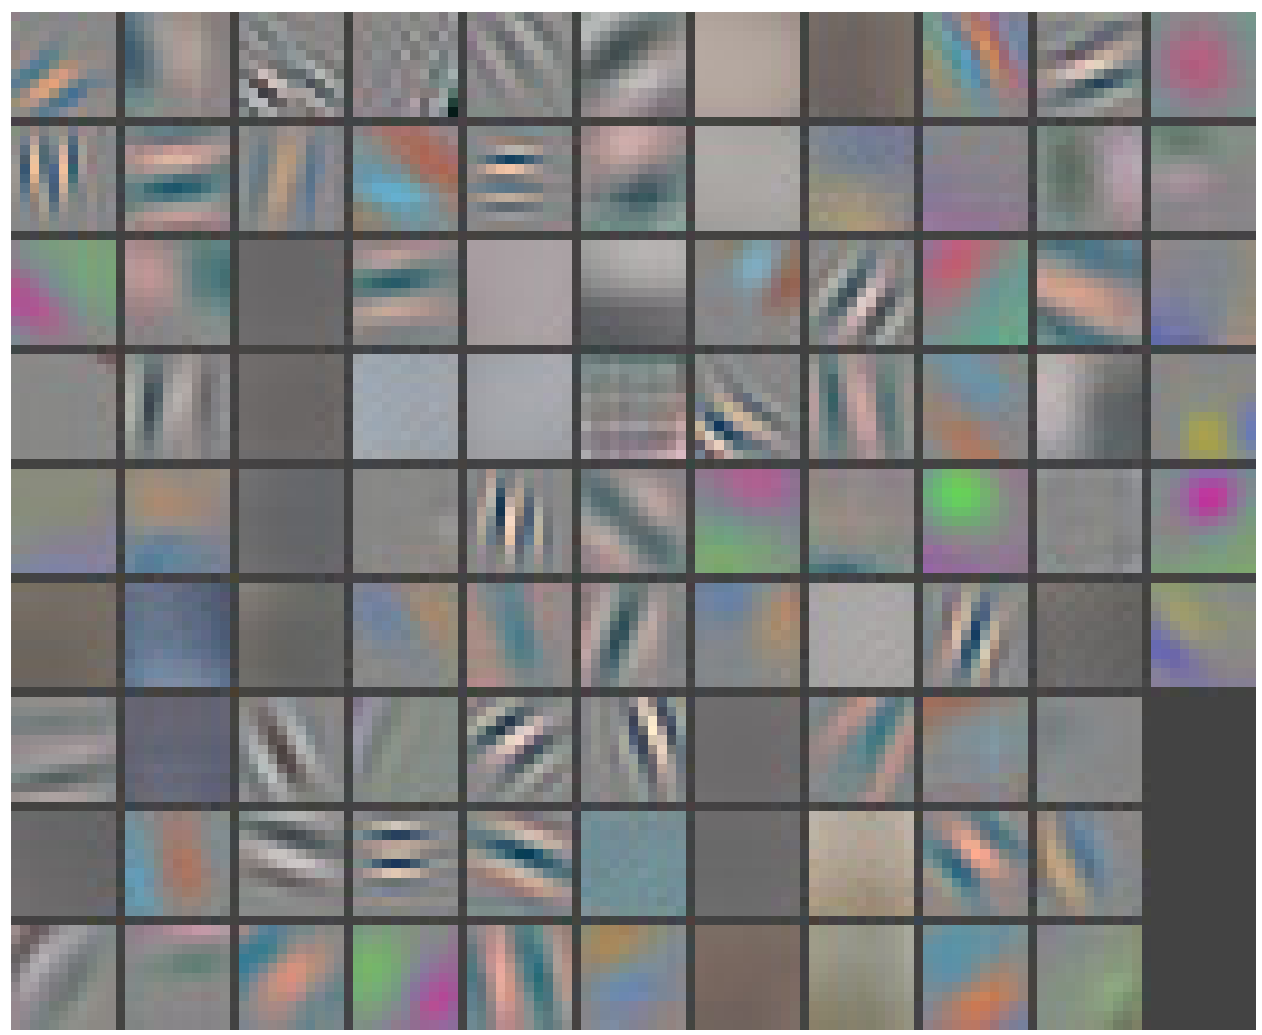
\includegraphics[width=0.55\linewidth]{./img/alexnet_stem.png}
        \caption{AlexNet}
    \end{subfigure}
    \begin{subfigure}{0.4\linewidth}
        \centering
        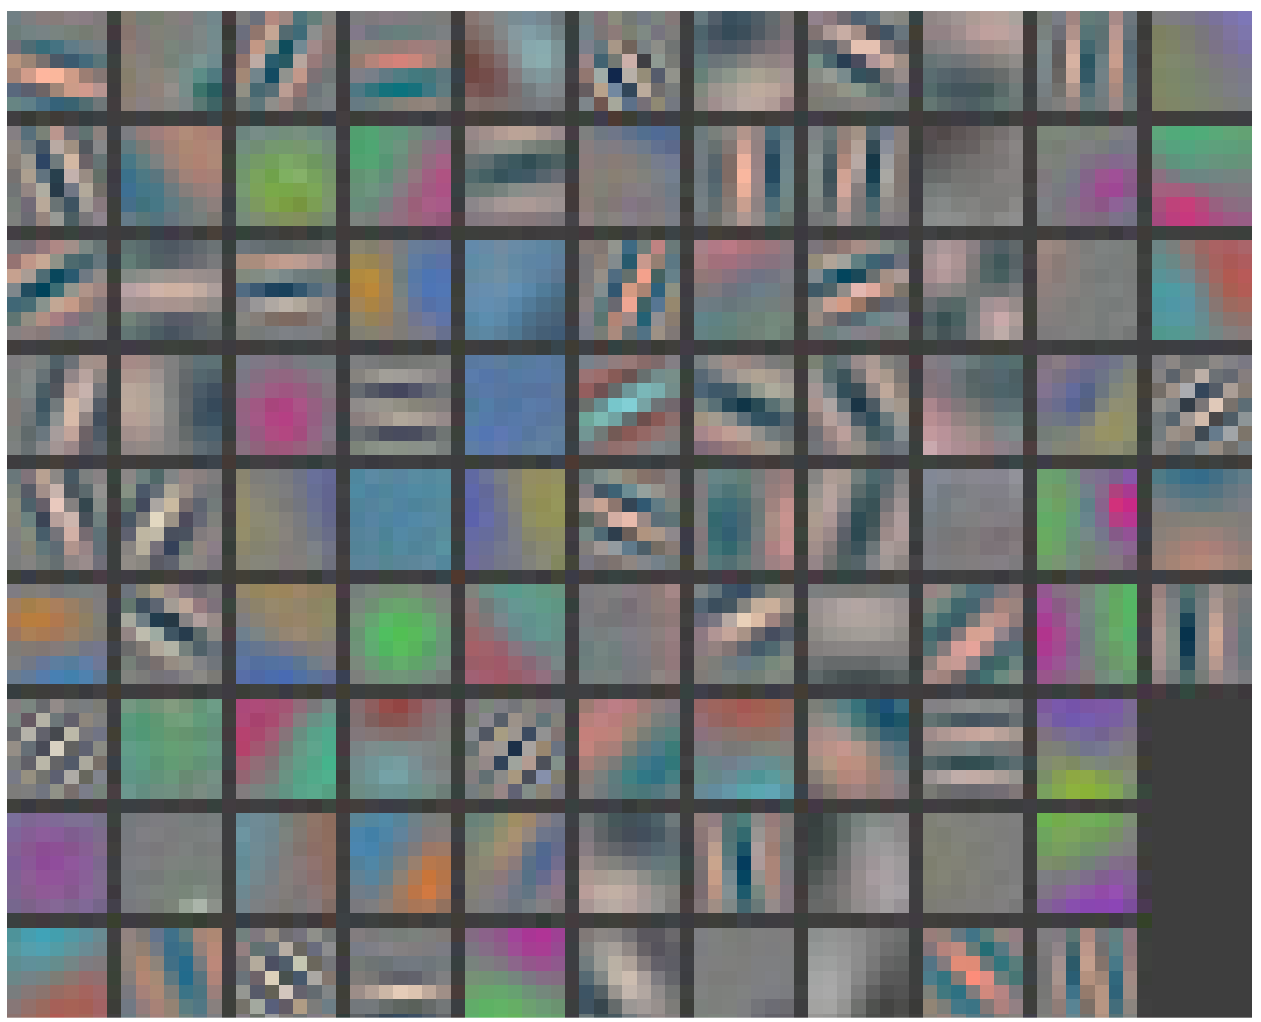
\includegraphics[width=0.55\linewidth]{./img/zfnet_stem.png}
        \caption{ZFNet}
    \end{subfigure}
    \caption{First layer activations comparison}
\end{figure}


\section{VGG}
\marginnote{VGG}


\subsection{Architecture}

Network with a higher depth and smaller components.
The authors constrained the layers to:
\begin{itemize}
    \item $3 \times 3$ convolutions with stride $1$ and padding $1$.
    \item $2 \times 2$ max-pooling with stride $2$ and padding $0$.
    \item Number of channels that doubles after each pool.
\end{itemize}

\begin{remark}
    It has been found out that deeper networks work better.
\end{remark}

\begin{description}
    \item[Stage] \marginnote{Stage}
        Fixed combination of layers that process inputs of the same spatial resolution.

        VGG stages are:
        \begin{itemize}
            \item $\texttt{conv} \mapsto \texttt{conv} \mapsto \texttt{pool}$.
            \item $\texttt{conv} \mapsto \texttt{conv} \mapsto \texttt{conv} \mapsto \texttt{pool}$.
            \item $\texttt{conv} \mapsto \texttt{conv} \mapsto \texttt{conv} \mapsto \texttt{conv} \mapsto \texttt{pool}$.
        \end{itemize}

        \begin{remark}
            One stage has the same receptive field of a single larger convolution but 
            has fewer parameters, requires less computation and adds more non-linearity.

            On the other hand, two activations are computed and both need to be stored for backpropagation.

            \indenttbox
            \begin{example}
                \phantom{}
                \begin{center}
                    \footnotesize
                    \begin{tabular}{cccc}
                        \toprule
                        \textbf{Convolutional layer} & \textbf{Parameters} & \textbf{FLOPs} & \textbf{Activations} \\
                        \midrule
                        $C \times C \times 5 \times 5$, $S=1$, $P=2$ & $25C^2 + C$ & $50C^2 \cdot W_\text{in} \cdot H_\text{in}$ & $C \cdot W_\text{in} \cdot H_\text{in}$ \\
                        Two stacked $C \times C \times 3 \times 3$, $S=1$, $P=1$ & $18C^2 + 2C$ & $36C^2 \cdot W_\text{in} \cdot H_\text{in}$ & $2 \cdot C \cdot W_\text{in} \cdot H_\text{in}$ \\
                        \bottomrule
                    \end{tabular}
                \end{center}
            \end{example}
        \end{remark}
\end{description}

\begin{remark}
    Local response normalization was experimented with and dropped.
    As batch normalization had not been invented yet, weights at deeper layers were initialized from shallower architectures.
\end{remark}

\begin{table}[H]
    \centering
    \caption{Architecture of various versions of VGG}
    \scriptsize
    \begin{tabular}{c|c|c|c|c|c}
        \toprule
        \makecell{\textbf{A}\\\tiny(11 weight layers)} &
        \makecell{\textbf{B}\\\tiny(11 weight layers)} &
        \makecell{\textbf{C}\\\tiny(13 weight layers)} &
        \makecell{\textbf{D}\\\tiny(16 weight layers)} &
        \makecell{\textbf{VGG-16}\\\tiny(16 weight layers)} &
        \makecell{\textbf{VGG-19}\\\tiny(19 weight layers)} \\
        \bottomrule
        \toprule
        \multicolumn{6}{c}{Input ($224 \times 224$ RGB image)} \\
        \midrule
        conv3-64 & conv3-64 & conv3-64 & conv3-64 & conv3-64 & conv3-64 \\
                 & LRN      & conv3-64 & conv3-64 & conv3-64 & conv3-64 \\
        \midrule
        \multicolumn{6}{c}{max-pool} \\
        \midrule
        conv3-128 & conv3-128 & conv3-128 & conv3-128 & conv3-128 & conv3-128 \\
                  &           & conv3-128 & conv3-128 & conv3-128 & conv3-128 \\
        \midrule
        \multicolumn{6}{c}{max-pool} \\
        \midrule
        conv3-256 & conv3-256 & conv3-256 & conv3-256 & conv3-256 & conv3-256 \\
        conv3-256 & conv3-256 & conv3-256 & conv3-256 & conv3-256 & conv3-256 \\
                  &           &           & conv1-256 & conv3-256 & conv3-256 \\
                  &           &           &           &           & conv3-256 \\
        \midrule
        \multicolumn{6}{c}{max-pool} \\
        \midrule
        conv3-512 & conv3-512 & conv3-512 & conv3-512 & conv3-512 & conv3-512 \\
        conv3-512 & conv3-512 & conv3-512 & conv3-512 & conv3-512 & conv3-512 \\
                  &           &           & conv1-512 & conv3-512 & conv3-512 \\
                  &           &           &           &           & conv3-512 \\
        \midrule
        \multicolumn{6}{c}{max-pool} \\
        \midrule
        conv3-512 & conv3-512 & conv3-512 & conv3-512 & conv3-512 & conv3-512 \\
        conv3-512 & conv3-512 & conv3-512 & conv3-512 & conv3-512 & conv3-512 \\
                  &           &           & conv1-512 & conv3-512 & conv3-512 \\
                  &           &           &           &           & conv3-512 \\
        \midrule
        \multicolumn{6}{c}{max-pool} \\
        \midrule
        \multicolumn{6}{c}{FC-4096} \\
        \multicolumn{6}{c}{FC-4096} \\
        \multicolumn{6}{c}{FC-1000} \\
        \multicolumn{6}{c}{\texttt{softmax}} \\
        \bottomrule
    \end{tabular}
\end{table}


\subsection{Properties}

VGG-16 has the following trends:
\begin{itemize}
    \item Most of the parameters are concentrated at the fully connected layers.
    \item Most of the computation is required by the convolutions.
    \item Most of the memory is required to store the activations as there are no stem layers.
    \item Training was done on 4 GPUs with data parallelism for 2-3 weeks.
\end{itemize}

\begin{table}[H]
    \centering
    \caption{Parameters of VGG-16 (batch size of 128)}
    \scriptsize
    \begin{tabular}{cccccccccccc}
        \toprule
        \multirow{2}[20]{*}{\textbf{Layer}} 
            & \multicolumn{4}{c}{\textbf{Convolution}} 
            & \multicolumn{3}{c}{\textbf{Single activation}} 
            & \multicolumn{2}{c}{\textbf{Batch requirements}}
            & \multicolumn{2}{c}{\textbf{Parameters}} \\
        \cmidrule(lr){2-5} \cmidrule(lr){6-8} \cmidrule(lr){9-10} \cmidrule(lr){11-12}
            & \rot{\textbf{Channels}} & \rot{\textbf{H/W}} & \rot{\textbf{Stride}} & \rot{\textbf{Padding}} 
            & \rot{\textbf{H/W}} & \rot{\textbf{Channels}} & \rot{\texttt{\#activations}} 
            & \rot{\textbf{MFLOPs}} & \rot{\textbf{Activ. mem.}} & \rot{\textbf{Amount}} & \rot{\textbf{Memory}} \\
        \midrule
        \texttt{input}   & --   & -- & -- & -- & 224 & \num{3}     & \num{150528}  & --             & \num{73.5} {\tiny MB}   & \num{0}                & \num{0.0}                \\
        \cmidrule(lr){1-12}
        \texttt{conv1}   & 64   & 3  & 1  & 1  & 224 & \num{64}    & \num{3211264} & \num{22196.3}  & \num{3136.0} {\tiny MB} & \num{2} {\tiny K}      & \num{0.0}                \\
        \texttt{conv2}   & 64   & 3  & 1  & 1  & 224 & \num{64}    & \num{3211264} & \num{473520.1} & \num{3136.0} {\tiny MB} & \num{37} {\tiny K}     & \num{0.4} {\tiny MB}     \\
        \texttt{pool1}   & 1    & 2  & 2  & 0  & 112 & \num{64}    & \num{802816}  & \num{411.0}    & \num{784.0} {\tiny MB}  & \num{0}                & \num{0.0}                \\
        \cmidrule(lr){1-12}
        \texttt{conv3}   & 128  & 3  & 1  & 1  & 112 & \num{128}   & \num{1605632} & \num{236760.1} & \num{1568.0} {\tiny MB} & \num{74} {\tiny K}     & \num{0.8} {\tiny MB}     \\
        \texttt{conv4}   & 128  & 3  & 1  & 1  & 112 & \num{128}   & \num{1605632} & \num{473520.1} & \num{1568.0} {\tiny MB} & \num{148} {\tiny K}    & \num{1.7} {\tiny MB}     \\
        \texttt{pool2}   & 1    & 2  & 2  & 0  & 56  & \num{128}   & \num{401408}  & \num{205.5}    & \num{392.0} {\tiny MB}  & \num{0}                & \num{0.0}                \\
        \cmidrule(lr){1-12}
        \texttt{conv5}   & 256  & 3  & 1  & 1  & 56  & \num{256}   & \num{802816}  & \num{236760.1} & \num{784.0} {\tiny MB}  & \num{295} {\tiny K}    & \num{3.4} {\tiny MB}     \\
        \texttt{conv6}   & 256  & 3  & 1  & 1  & 56  & \num{256}   & \num{802816}  & \num{473520.1} & \num{784.0} {\tiny MB}  & \num{590} {\tiny K}    & \num{6.8} {\tiny MB}     \\
        \texttt{conv7}   & 256  & 3  & 1  & 1  & 56  & \num{256}   & \num{802816}  & \num{473520.1} & \num{784.0} {\tiny MB}  & \num{590} {\tiny K}    & \num{6.8} {\tiny MB}     \\
        \texttt{pool3}   & 1    & 2  & 2  & 0  & 28  & \num{256}   & \num{200704}  & \num{102.8}    & \num{196.0} {\tiny MB}  & \num{0}                & \num{0.0}                \\
        \cmidrule(lr){1-12}
        \texttt{conv8}   & 512  & 3  & 1  & 1  & 28  & \num{512}   & \num{401408}  & \num{236760.1} & \num{392.0} {\tiny MB}  & \num{1180} {\tiny K}   & \num{13.5} {\tiny MB}    \\
        \texttt{conv9}   & 512  & 3  & 1  & 1  & 28  & \num{512}   & \num{401408}  & \num{473520.1} & \num{392.0} {\tiny MB}  & \num{2360} {\tiny K}   & \num{27.0} {\tiny MB}    \\
        \texttt{conv10}  & 512  & 3  & 1  & 1  & 28  & \num{512}   & \num{401408}  & \num{473520.1} & \num{392.0} {\tiny MB}  & \num{2360} {\tiny K}   & \num{27.0} {\tiny MB}    \\
        \texttt{pool4}   & 1    & 2  & 2  & 0  & 14  & \num{512}   & \num{100352}  & \num{51.4}     & \num{98.0} {\tiny MB}   & \num{0}                & \num{0.0}                \\
        \cmidrule(lr){1-12}
        \texttt{conv11}  & 512  & 3  & 1  & 1  & 14  & \num{512}   & \num{100352}  & \num{118380.0} & \num{98.0} {\tiny MB}   & \num{2360} {\tiny K}   & \num{27.0} {\tiny MB}    \\
        \texttt{conv12}  & 512  & 3  & 1  & 1  & 14  & \num{512}   & \num{100352}  & \num{118380.0} & \num{98.0} {\tiny MB}   & \num{2360} {\tiny K}   & \num{27.0} {\tiny MB}    \\
        \texttt{conv13}  & 512  & 3  & 1  & 1  & 14  & \num{512}   & \num{100352}  & \num{118380.0} & \num{98.0} {\tiny MB}   & \num{2360} {\tiny K}   & \num{27.0} {\tiny MB}    \\
        \texttt{pool5}   & 1    & 2  & 2  & 0  & 7   & \num{512}   & \num{25088}   & \num{12.8}     & \num{24.5} {\tiny MB}   & \num{0}                & \num{0.0}                \\
        \cmidrule(lr){1-12}
        \texttt{flatten} & 1    & 1  & 1  & 0  & 1   & \num{25088} & \num{25088}   & \num{0.0}      & \num{0.0}               & \num{0}                & \num{0.0}                \\
        \texttt{fc14}    & 4096 & 1  & 1  & 0  & 1   & \num{4096}  & \num{4096}    & \num{26306.7}  & \num{4.0} {\tiny MB}    & \num{102786} {\tiny K} & \num{1176.3} {\tiny MB}  \\
        \texttt{fc15}    & 4096 & 1  & 1  & 0  & 1   & \num{4096}  & \num{4096}    & \num{4295.0}   & \num{4.0} {\tiny MB}    & \num{16781} {\tiny K}  & \num{192.0} {\tiny MB}   \\
        \texttt{fc16}    & 1000 & 1  & 1  & 0  & 1   & \num{1000}  & \num{1000}    & \num{1048.6}   & \num{1.0} {\tiny MB}    & \num{4100} {\tiny K}   & \num{46.9} {\tiny MB}    \\
        \midrule
        &&&&&&& \textbf{Total} & \num{3961171} & \num{14733} {\tiny MB} & \num{138382} {\tiny K} & \num{1584} {\tiny MB} \\
        \bottomrule
    \end{tabular}
\end{table}



\section{Inception-v1 (GoogLeNet)}
\marginnote{Inception-v1 (GoogLeNet)}

Network that aims to optimize computing resources.


\subsection{Architecture}

\begin{description}
    \item[Stem layers]
        Down-sample the image from a shape of 224 to 28.
        As in ZFNet, multiple layers are used (5) and the largest convolution is of shape $7 \times 7$ with stride $2$.

    \item[Inception module] \marginnote{Inception module}
        Main component of Inception-v1 that computes multiple convolutions on the input.

        \begin{description}
            \item[Naive approach] 
                Given the input, the output is the concatenation of:
                \begin{itemize}
                    \item A $5 \times 5$ convolution with stride $1$ and padding $2$.
                    \item A $3 \times 3$ convolution with stride $1$ and padding $1$.
                    \item A $1 \times 1$ convolution with stride $1$ and padding $0$.
                    \item A $3 \times 3$ max-pooling with stride $1$ and padding $1$.
                \end{itemize} 

                By using this approach, two problems arise:
                \begin{itemize}
                    \item The max-pooling layer outputs a large number of channels (same as input).
                    \item The convolutions are computationally expensive due to the large number of input channels.
                \end{itemize}

                \begin{figure}[H]
                    \centering
                    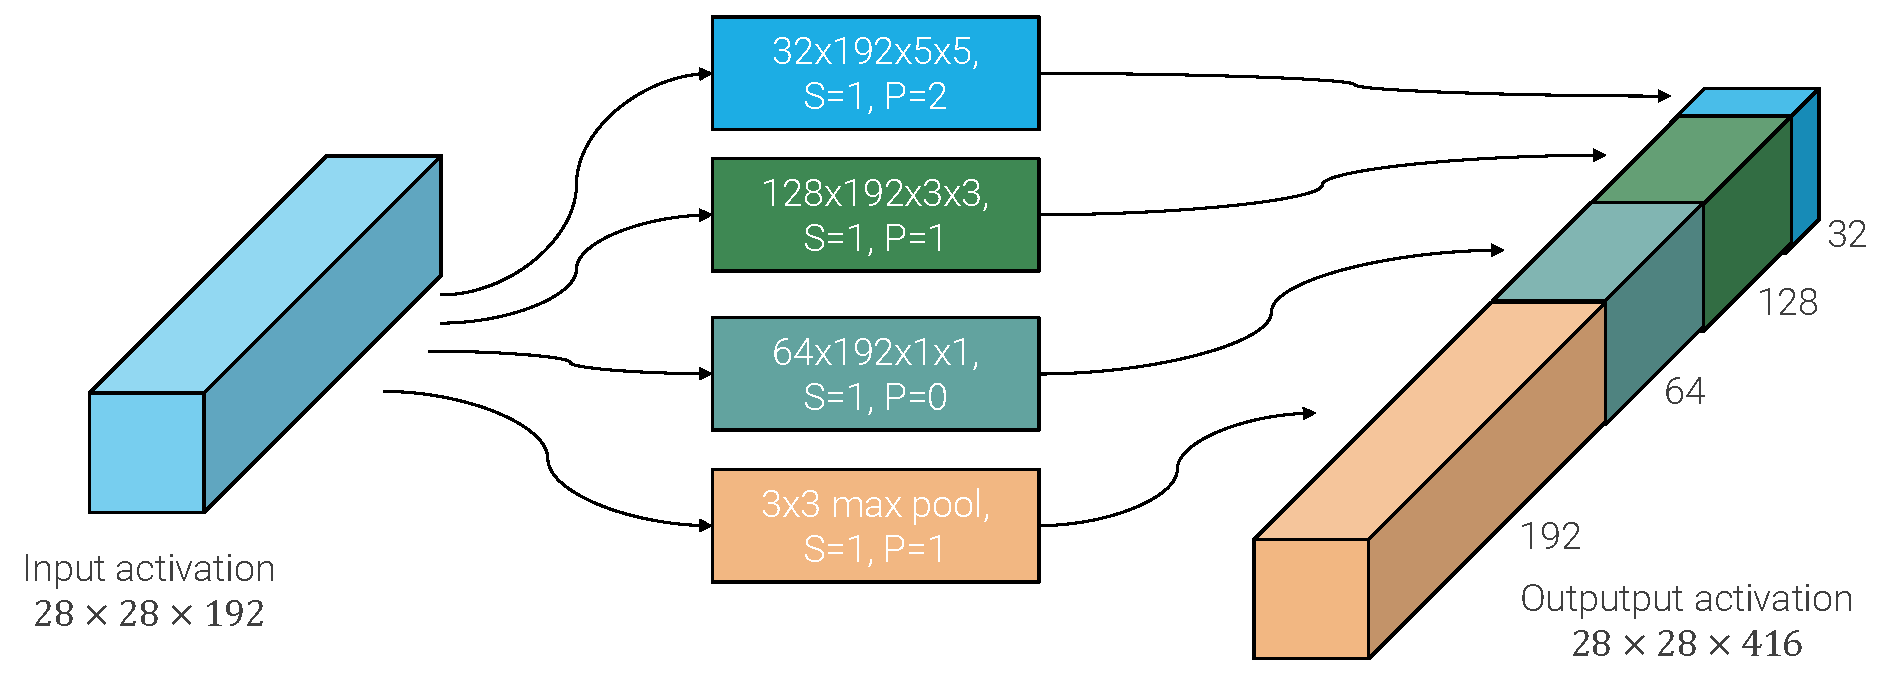
\includegraphics[width=0.65\linewidth]{./img/_naive_inception.pdf}
                    \caption{Naive inception module on the output of the stem layers}
                \end{figure}
                
                
            \item[Actual approach] 
                Same as the naive approach, but max-pooling, $5 \times 5$ and $3 \times 3$ convolutions
                are preceded by $1 \times 1$ convolutions.
                
                \begin{remark}
                    For max-pooling, the $1 \times 1$ convolution can indifferently be placed before or after.    
                \end{remark}

                \begin{figure}[H]
                    \centering
                    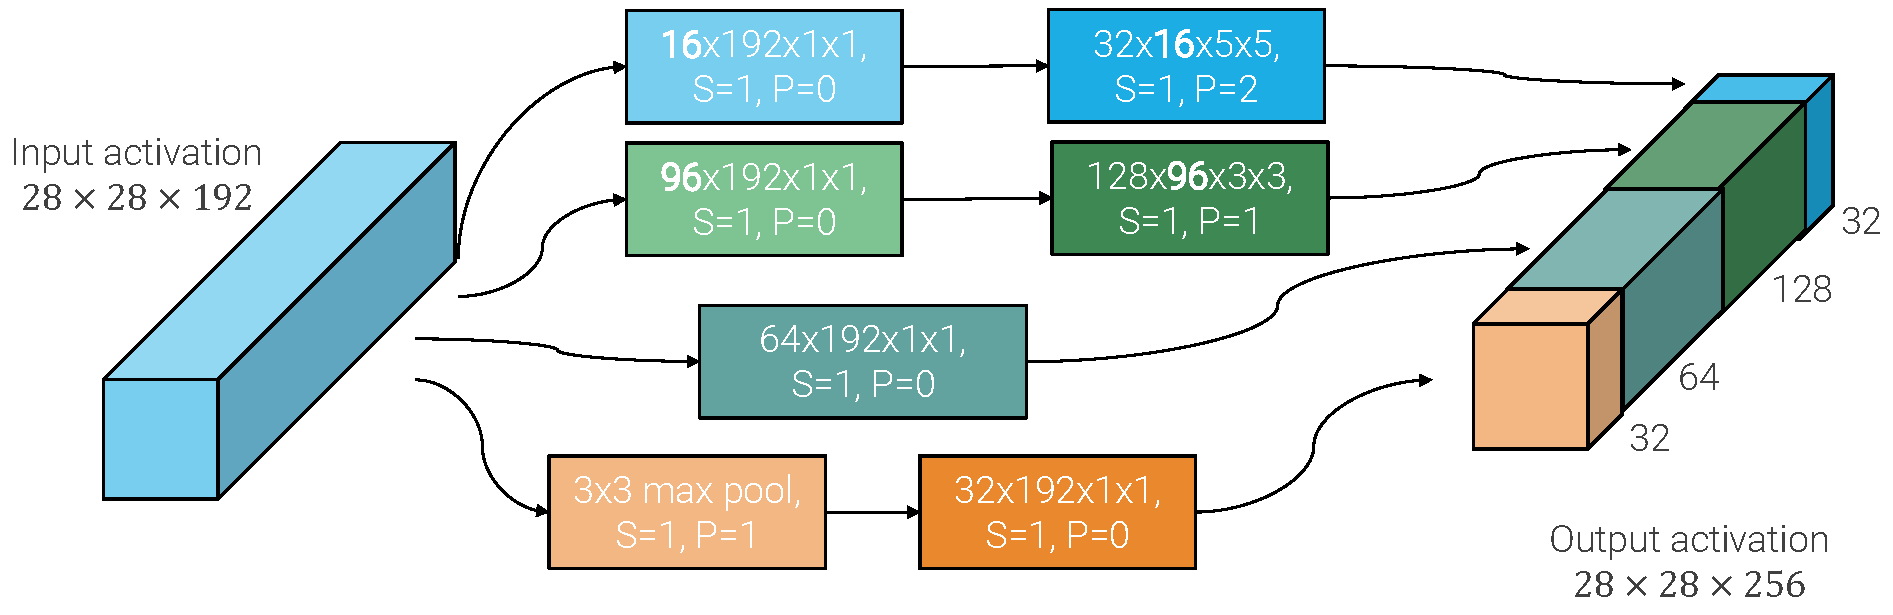
\includegraphics[width=0.65\linewidth]{./img/_actual_inception.pdf}
                    \caption{Actual inception module on the output of the stem layers}
                \end{figure}
            \end{description}
        \begin{remark}
            The multiple convolutions of an inception module can be seen as decision components.
        \end{remark}

    \item[Auxiliary \texttt{softmax}]
        Intermediate \texttt{softmax}s are used to ensure that hidden features are good enough.
        They also act as regularizers.

        During inference, they are discarded.

    \item[Global average pooling classifier] \marginnote{Global average pooling classifier}
        Instead of flattening between the convolutional and fully connected layers, 
        global average pooling is used to reduce the number of parameters.

        \begin{remark}
            If the kernel size of the pooling layer is computed by the layer itself (e.g. \texttt{AdaptiveAvgPool2d}), 
            the network will be able to process inputs of any size (but this does not guarantee the quality of classification for all the image shapes).
        \end{remark}
    
\end{description}

\begin{figure}[H]
    \centering
    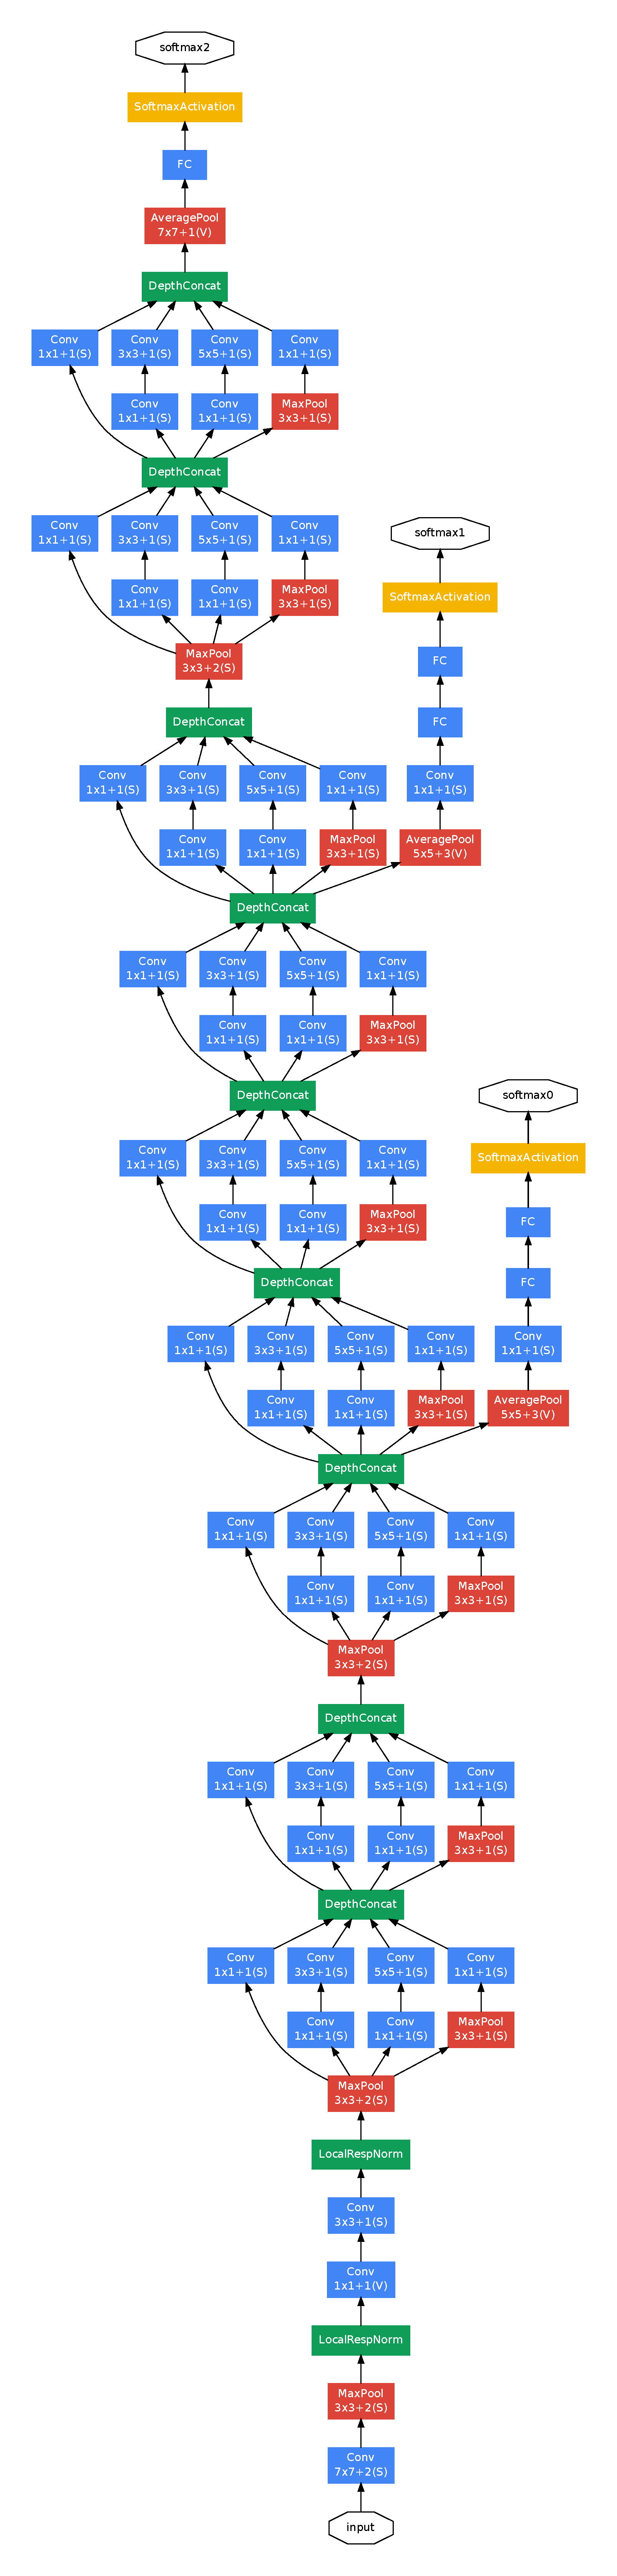
\includegraphics[angle=-90, width=0.85\linewidth]{./img/_inception_v1.pdf}
    \caption{Architecture of Inception-v1}
\end{figure}


\subsection{Properties}

\begin{itemize}
    \item The fully connected layer has a relatively small amount of parameters and a negligible number of FLOPs.
    \item Metrics were measured using test-time augmentation 
        (the input image is split into random small chunks and each is processed by the network separately. The final result is the average of the results as in ensemble models).
        Strictly speaking, this makes results difficult to compare to other models that only do a single pass.
\end{itemize}

\begin{table}[H]
    \centering
    \caption{Parameters of Inception-v1 (batch size of 128)}
    \scriptsize
    \setlength{\tabcolsep}{2pt}
    \begin{tabular}{cccccccccccccccccccc}
        \toprule
        \multirow{2}[20]{*}{\textbf{Layer}} 
            & \multicolumn{4}{c}{\makecell{ \textbf{Incep. $1 \times 1$}\\\textbf{Other conv.} }}
            & \multicolumn{3}{c}{\textbf{Incep. $3 \times 3$}} 
            & \multicolumn{3}{c}{\textbf{Incep. $5 \times 5$}} 
            & \multicolumn{2}{c}{\textbf{Max-pool}} 
            & \multicolumn{3}{c}{\textbf{Single activ.}} 
            & \multicolumn{2}{c}{\textbf{Batch requir.}}
            & \multicolumn{2}{c}{\textbf{Parameters}} \\
        \cmidrule(lr){2-5} \cmidrule(lr){6-8} \cmidrule(lr){9-11} \cmidrule(lr){12-13} \cmidrule(lr){14-16} \cmidrule(lr){17-18} \cmidrule(lr){19-20}
            & \rot{\textbf{Channels}} & \rot{\textbf{H/W}} & \rot{\textbf{Stride}} & \rot{\textbf{Padding}} 
            & \rot{\textbf{Channels}} & \rot{\textbf{$1 \times 1$ ch.s}} & \rot{\textbf{H/W}}
            & \rot{\textbf{Channels}} & \rot{\textbf{$1 \times 1$ ch.s}} & \rot{\textbf{H/W}}
            & \rot{\textbf{$1 \times 1$ ch.s}} & \rot{\textbf{H/W}}
            & \rot{\textbf{H/W}} & \rot{\textbf{Channels}} & \rot{\texttt{\#activations}}
            & \rot{\textbf{MFLOPs}} & \rot{\textbf{Activ. mem.}} & \rot{\textbf{Amount}} & \rot{\textbf{Memory}} \\
        \midrule
        \texttt{input}   & --   & -- & -- & -- & --  & --  & -- & --  & --  & -- & --  & -- & 224 & \num{3}    & \num{150528} & --            & \num{73.5} {\tiny MB}  & \num{0}              & \num{0.0}             \\
        \cmidrule(lr){1-20}
        \texttt{conv1}   & 64   & 7  & 2  & 3  & --  & --  & -- & --  & --  & -- & --  & -- & 112 & \num{64}   & \num{802816} & \num{30211.6} & \num{784.0} {\tiny MB} & \num{9} {\tiny K}    & \num{0.1} {\tiny MB}  \\
        \texttt{pool1}   & 1    & 3  & 2  & 1  & --  & --  & -- & --  & --  & -- & --  & -- & 56  & \num{64}   & \num{200704} & \num{231.2}   & \num{196.0} {\tiny MB} & \num{0}              & \num{0.0}             \\
        \texttt{conv2}   & 64   & 1  & 1  & 0  & --  & --  & -- & --  & --  & -- & --  & -- & 56  & \num{64}   & \num{200704} & \num{3288.3}  & \num{196.0} {\tiny MB} & \num{4} {\tiny K}    & \num{0.0}             \\
        \texttt{conv3}   & 192  & 3  & 1  & 1  & --  & --  & -- & --  & --  & -- & --  & -- & 56  & \num{192}  & \num{602112} & \num{88785.0} & \num{588.0} {\tiny MB} & \num{111} {\tiny K}  & \num{1.3} {\tiny MB}  \\
        \cmidrule(lr){1-20}
        \texttt{pool2}   & 1    & 3  & 2  & 1  & --  & --  & -- & --  & --  & -- & --  & -- & 28  & \num{192}  & \num{150528} & \num{173.4}   & \num{147.0} {\tiny MB} & \num{0}              & \num{0.0}             \\
        \texttt{incep1}  & 64   & 1  & 1  & 0  & 128 & 96  & 3  & 32  & 16  & 5  & 32  & 3  & 28  & \num{256}  & \num{200704} & \num{31380.5} & \num{196.0} {\tiny MB} & \num{163} {\tiny K}  & \num{1.9} {\tiny MB}  \\
        \texttt{incep2}  & 128  & 1  & 1  & 0  & 192 & 128 & 3  & 96  & 32  & 5  & 64  & 3  & 28  & \num{480}  & \num{376320} & \num{75683.1} & \num{367.5} {\tiny MB} & \num{388} {\tiny K}  & \num{4.4} {\tiny MB}  \\
        \texttt{pool3}   & 1    & 3  & 2  & 1  & --  & --  & -- & --  & --  & -- & --  & -- & 14  & \num{480}  & \num{94080}  & \num{108.4}   & \num{91.9} {\tiny MB}  & \num{0}              & \num{0.0}             \\
        \texttt{incep3}  & 192  & 1  & 1  & 0  & 208 & 96  & 3  & 48  & 16  & 5  & 64  & 3  & 14  & \num{512}  & \num{100352} & \num{17403.4} & \num{98.0} {\tiny MB}  & \num{376} {\tiny K}  & \num{4.3} {\tiny MB}  \\
        \texttt{incep4}  & 160  & 1  & 1  & 0  & 224 & 112 & 3  & 64  & 24  & 5  & 64  & 3  & 14  & \num{512}  & \num{100352} & \num{20577.8} & \num{98.0} {\tiny MB}  & \num{449} {\tiny K}  & \num{5.1} {\tiny MB}  \\
        \texttt{incep5}  & 128  & 1  & 1  & 0  & 256 & 128 & 3  & 64  & 24  & 5  & 64  & 3  & 14  & \num{512}  & \num{100352} & \num{23609.2} & \num{98.0} {\tiny MB}  & \num{509} {\tiny K}  & \num{5.8} {\tiny MB}  \\
        \texttt{incep5}  & 112  & 1  & 1  & 0  & 288 & 144 & 3  & 64  & 32  & 5  & 64  & 3  & 14  & \num{528}  & \num{103488} & \num{28233.4} & \num{101.1} {\tiny MB} & \num{605} {\tiny K}  & \num{6.9} {\tiny MB}  \\
        \texttt{incep6}  & 256  & 1  & 1  & 0  & 320 & 160 & 3  & 128 & 32  & 5  & 128 & 3  & 14  & \num{832}  & \num{163072} & \num{41445.4} & \num{159.3} {\tiny MB} & \num{867} {\tiny K}  & \num{9.9} {\tiny MB}  \\
        \texttt{pool4}   & 1    & 3  & 2  & 1  & --  & --  & -- & --  & --  & -- & --  & -- & 7   & \num{832}  & \num{40768}  & \num{47.0}    & \num{39.8} {\tiny MB}  & \num{0}              & \num{0.0}             \\
        \texttt{incep7}  & 256  & 1  & 1  & 0  & 320 & 160 & 3  & 128 & 32  & 5  & 128 & 3  & 7   & \num{832}  & \num{40768}  & \num{11860.0} & \num{39.8} {\tiny MB}  & \num{1042} {\tiny K} & \num{11.9} {\tiny MB} \\
        \texttt{incep8}  & 384  & 1  & 1  & 0  & 384 & 192 & 3  & 128 & 48  & 5  & 128 & 3  & 7   & \num{1024} & \num{50176}  & \num{16689.7} & \num{49.0} {\tiny MB}  & \num{1443} {\tiny K} & \num{16.5} {\tiny MB} \\
        \cmidrule(lr){1-20}
        \texttt{avgpool} & 1    & 1  & 1  & 0  & --  & --  & -- & --  & --  & -- & --  & -- & 1   & \num{1024} & \num{1024}   & \num{6.4}     & \num{1.0} {\tiny MB}   & \num{0}              & \num{0.0}             \\
        \texttt{fc1}     & 1000 & 1  & 1  & 0  & --  & --  & -- & --  & --  & -- & --  & -- & 1   & \num{1000} & \num{1000}   & \num{262.1}   & \num{1.0} {\tiny MB}   & \num{1025} {\tiny K} & \num{11.7} {\tiny MB} \\
        \midrule
        &&&&&&&&&&&&&&& \textbf{Total} & \num{389996} & \num{3251} {\tiny MB} & \num{6992} {\tiny K} & \num{80} {\tiny MB} \\
        \bottomrule
    \end{tabular}
\end{table}


\subsection{Inception-v3}
\marginnote{Inception-v3}

Uses convolution factorization to improve computational efficiency, reduce the number of parameters and make training more disentangled and easier.
Different modules are used depending on the activation shape.

\begin{figure}[H]
    \centering
    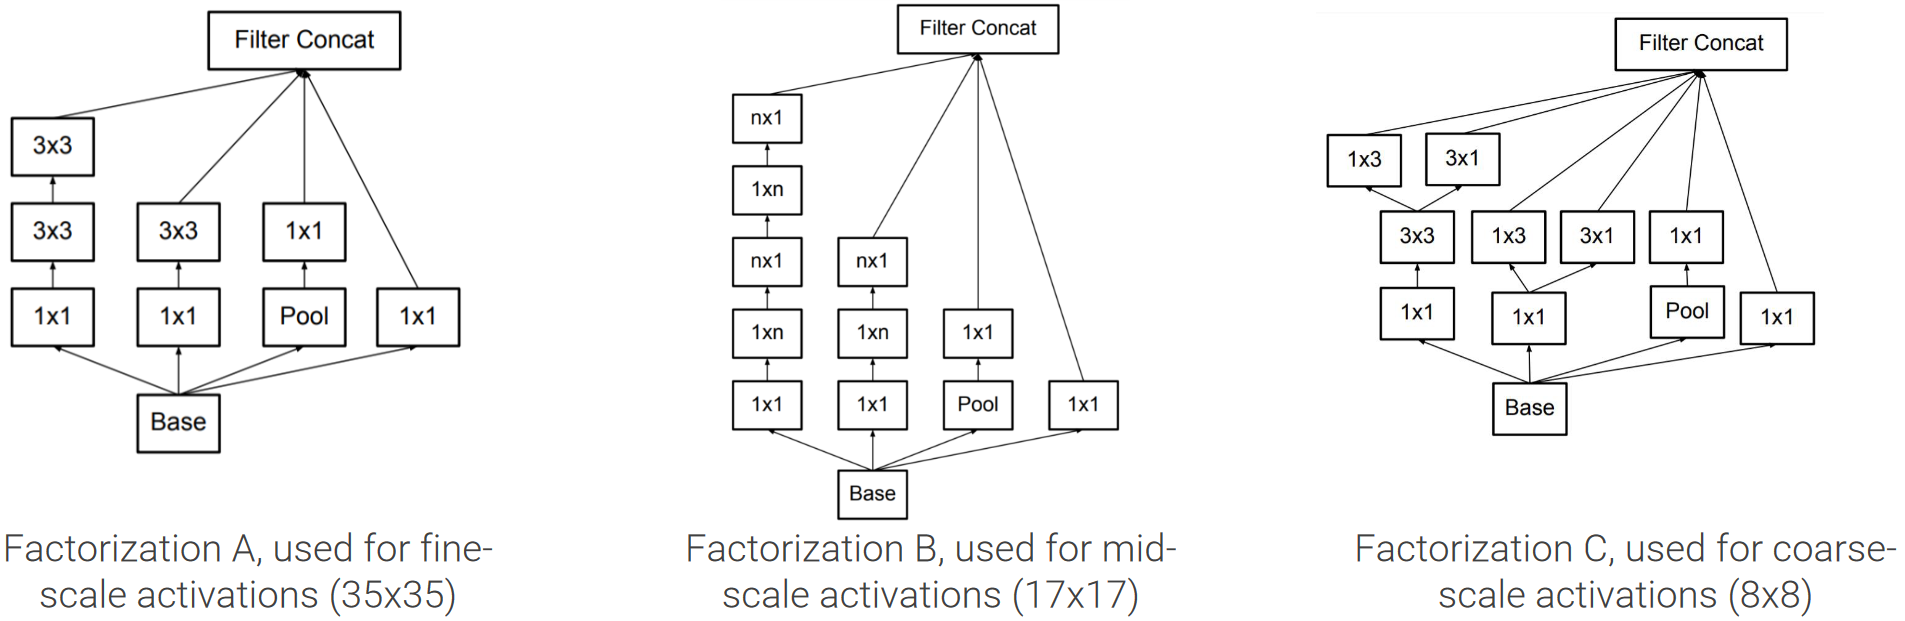
\includegraphics[width=0.75\linewidth]{./img/inception_v3.png}
    \caption{Inception-v3 modules}
\end{figure}


\subsection{Inception-v4}
\marginnote{Inception-v4}

A larger version of Inception v3 with more complicated stem layers.



\section{Residual networks}

\begin{remark}
    Training a very deep network from scratch might result in a solution that performs worse than a shallower layer.
    One could expect that the network simply overfits, but in reality, it underfits as gradient descent is not able to find a solution.

    \begin{figure}[H]
        \centering
        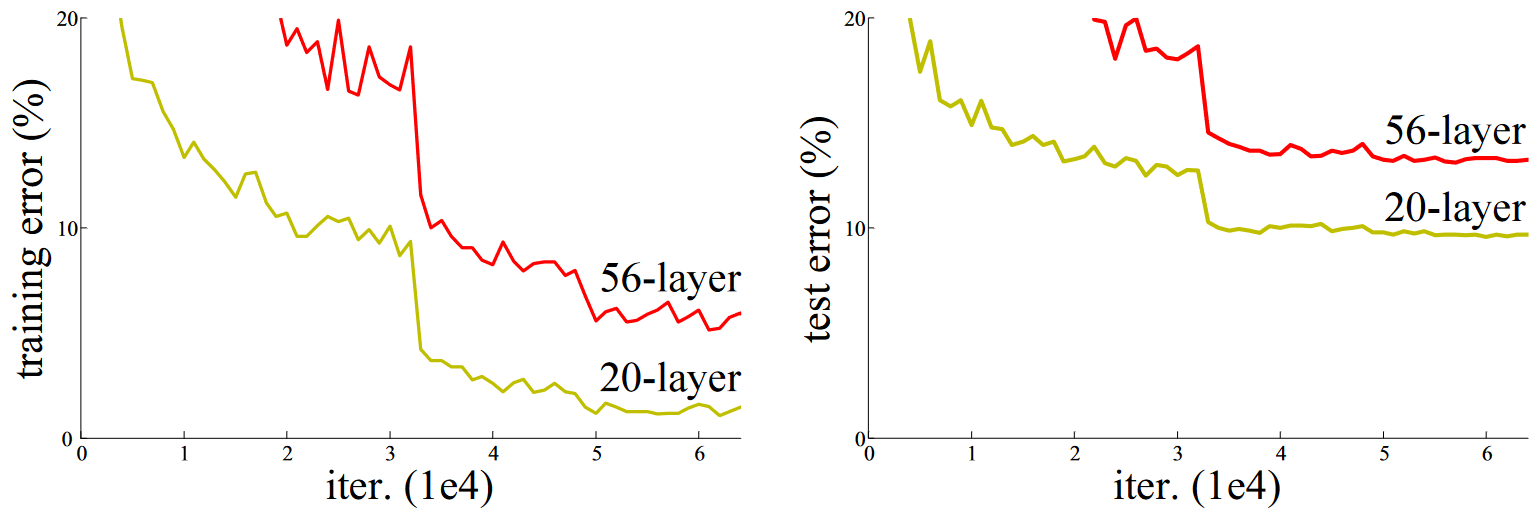
\includegraphics[width=0.5\linewidth]{./img/deep_network_error.png}
    \end{figure}
\end{remark}

\begin{remark}
    Technically, a deep neural network that has similar performance to a small network $\mathcal{N}$ can always be constructed.
    It is sufficient to take $\mathcal{N}$ as the starting network and add an arbitrary amount of identity layers.
\end{remark}

\begin{description}
    \item[Standard residual block] \marginnote{Standard residual block}
        Block that allows to easily learn the identity function through a skip connection.
        The output of a residual block with input $x$ and a series of convolutional layers $F$ is:
        \[ F(x; \matr{\theta}) + x \]

        \begin{minipage}{0.75\linewidth}
            \begin{description}
                \item[Skip connection] \marginnote{Skip connection}
                    Connection that skips a certain number of layers (e.g. 2 convolutional blocks).
            \end{description}
    
            \begin{remark}
                Training starts with small weights so that the network starts as the identity function. Updates can be seen as perturbations of the identity function.
            \end{remark}
    
            \begin{remark}
                Batch normalization is heavily used.
            \end{remark}
        \end{minipage}
        \begin{minipage}{0.2\linewidth}
            \centering
            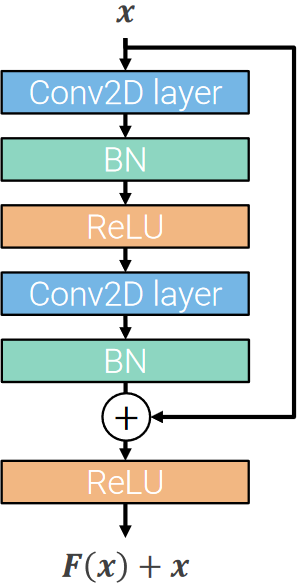
\includegraphics[width=0.8\linewidth]{./img/skip_conn.png}
        \end{minipage}
        
        \begin{remark}
            Skip connections are applied before the activation function (ReLU) as otherwise it would be summed to all positive values making the perturbation of the identity function less effective.
        \end{remark}
\end{description}


\subsection{ResNet}
\marginnote{ResNet-18}

VGG-inspired network with residual blocks.
It has the following properties:
\begin{itemize}
    \item A stage is composed of residual blocks.
    \item A residual block is composed of two $3 \times 3$ convolutions followed by batch normalization.
    \item The first residual block of each stage halves the spatial dimension and doubles the number of channels (there is no pooling).
    \item Stem layers are less aggressive than GoogLeNet (\texttt{conv + pool}. Input reduced to $56 \times 56$).
    \item Global average pooling is used instead of flattening.
\end{itemize}

\begin{figure}[H]
    \centering
    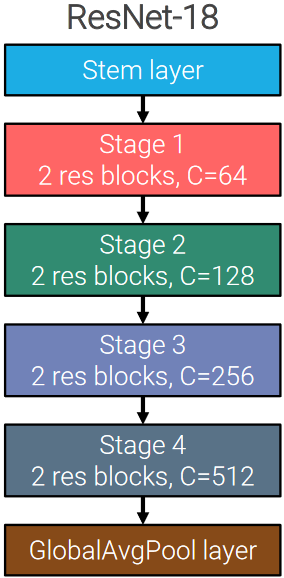
\includegraphics[width=0.15\linewidth]{./img/resnet_18.png}
    \caption{Architecture of ResNet-18}
\end{figure}

\begin{description}
    \item[Skip connection reshape]
        Due to the shape mismatch, the output of a stage cannot be directly used as the skip connection of the next stage.
        Possible solutions are:
        \begin{itemize}
            \item Apply stride $2$ and zero-pad the missing channels of the skip connection (this does not add new parameters).
            \item The output of the previous stage is passed through a $1 \times 1$ convolution with stride $2$ and $2C$ output channels (shown to work slightly better).
        \end{itemize}

    \item[Bottleneck residual network] \marginnote{Bottleneck residual network}
        Variant of residual blocks that uses more layers with approximately the same number of parameters and FLOPs of the standard residual block.
        Instead of using two $3 \times 3$ convolutions, bottleneck residual network has the following structure:
        \begin{itemize}
            \item $1 \times 1$ convolution to compress the channels of the input by an order of $4$ (and the spatial dimension by $2$ if it is the first block of a stage, as in the normal ResNet).
            \item $3 \times 3$ convolution.
            \item $1 \times 1$ convolution to match the shape of the skip connection.
        \end{itemize}

        \begin{figure}[H]
            \centering
            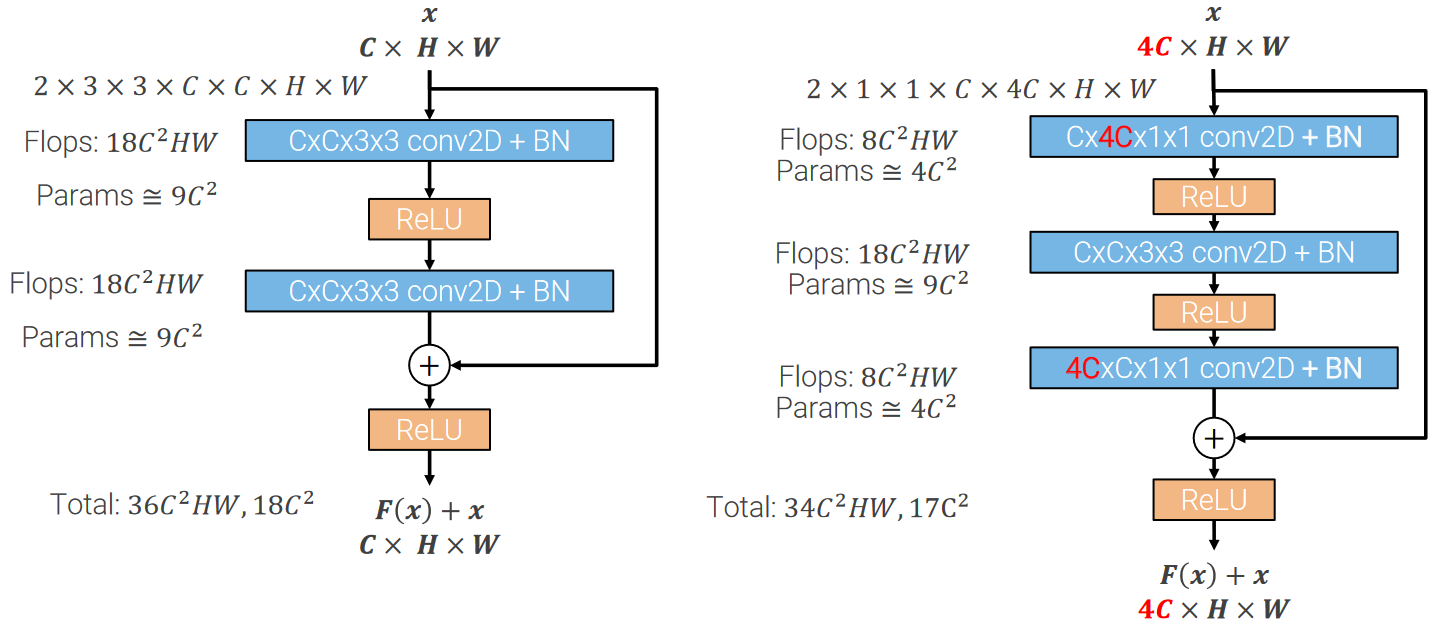
\includegraphics[width=0.7\linewidth]{./img/bottleneck_block.png}
            \caption{Standard residual block (left) and bottleneck block (right)}
        \end{figure}
\end{description}

\begin{remark}
    ResNet improves the results of a deeper layer but beyond a certain depth, the gain is negligible.
    \begin{figure}[H]
        \centering
        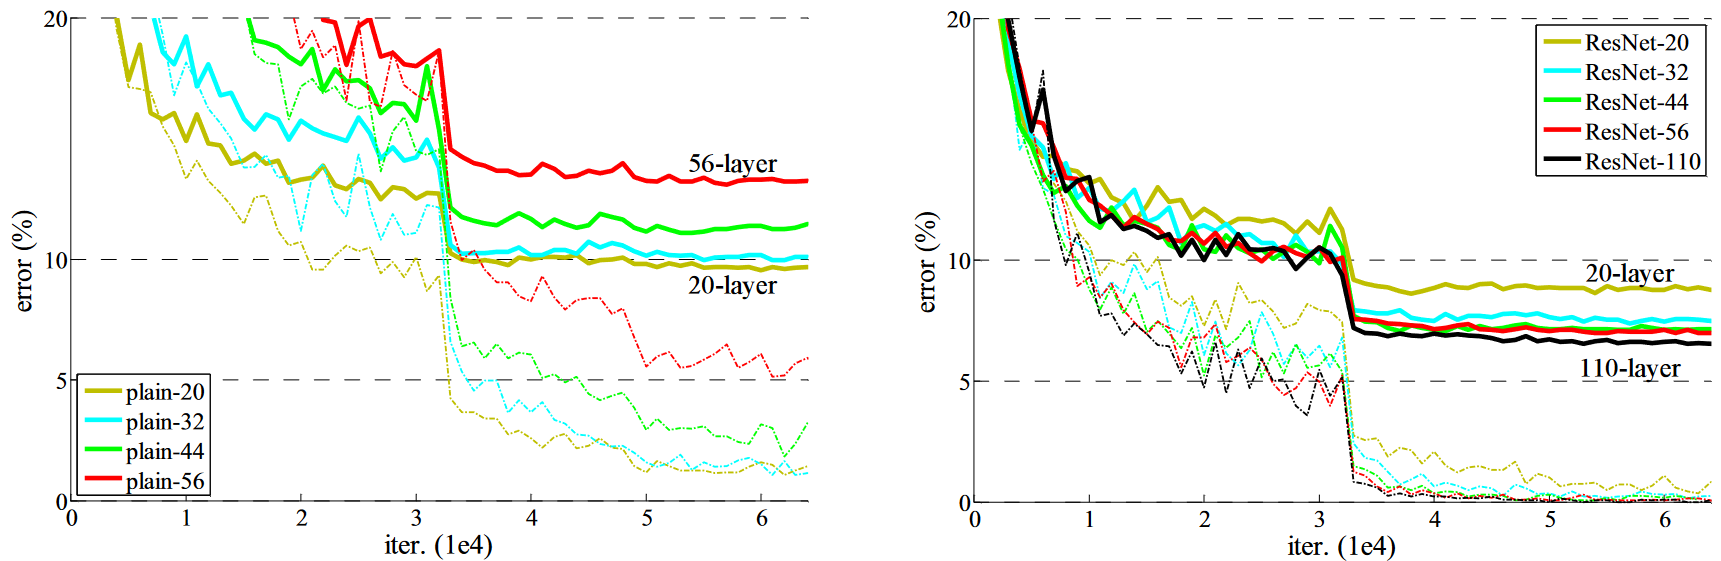
\includegraphics[width=0.65\linewidth]{./img/resnet_results.png}
    \end{figure}
\end{remark}

\begin{table}[H]
    \centering
    \caption{Variants of ResNet}
    \scriptsize
    \begin{tabular}{c|c|c|c|c}
        \toprule
        \textbf{ResNet-18} & \textbf{ResNet-34} & \textbf{ResNet-50} & \textbf{ResNet-101} & \textbf{ResNet-152} \\
        \bottomrule
        \toprule
        \multicolumn{5}{c}{Stem layers} \\
        \midrule
            \makecell{2 residual blocks\\($C=64$)} & 
            \makecell{3 residual blocks\\($C=64$)} & 
            \makecell{3 bottleneck blocks\\($C=256$)} & 
            \makecell{3 bottleneck blocks\\($C=256$)} & 
            \makecell{3 bottleneck blocks\\($C=256$)} \\
        \midrule
            \makecell{2 residual blocks\\($C=128$)} & 
            \makecell{4 residual blocks\\($C=128$)} & 
            \makecell{4 bottleneck blocks\\($C=512$)} & 
            \makecell{4 bottleneck blocks\\($C=512$)} & 
            \makecell{8 bottleneck blocks\\($C=512$)} \\
        \midrule
            \makecell{2 residual blocks\\($C=256$)} & 
            \makecell{6 residual blocks\\($C=256$)} & 
            \makecell{6 bottleneck blocks\\($C=1024$)} & 
            \makecell{23 bottleneck blocks\\($C=1024$)} & 
            \makecell{36 bottleneck blocks\\($C=1024$)} \\
        \midrule
            \makecell{2 residual blocks\\($C=512$)} & 
            \makecell{3 residual blocks\\($C=512$)} & 
            \makecell{3 bottleneck blocks\\($C=2048$)} & 
            \makecell{3 bottleneck blocks\\($C=2048$)} & 
            \makecell{3 bottleneck blocks\\($C=2048$)} \\
        \midrule
        \multicolumn{5}{c}{Average pooling + Fully-connected} \\
        \bottomrule
    \end{tabular}
\end{table}

% \begin{figure}[H]
%     \centering
%     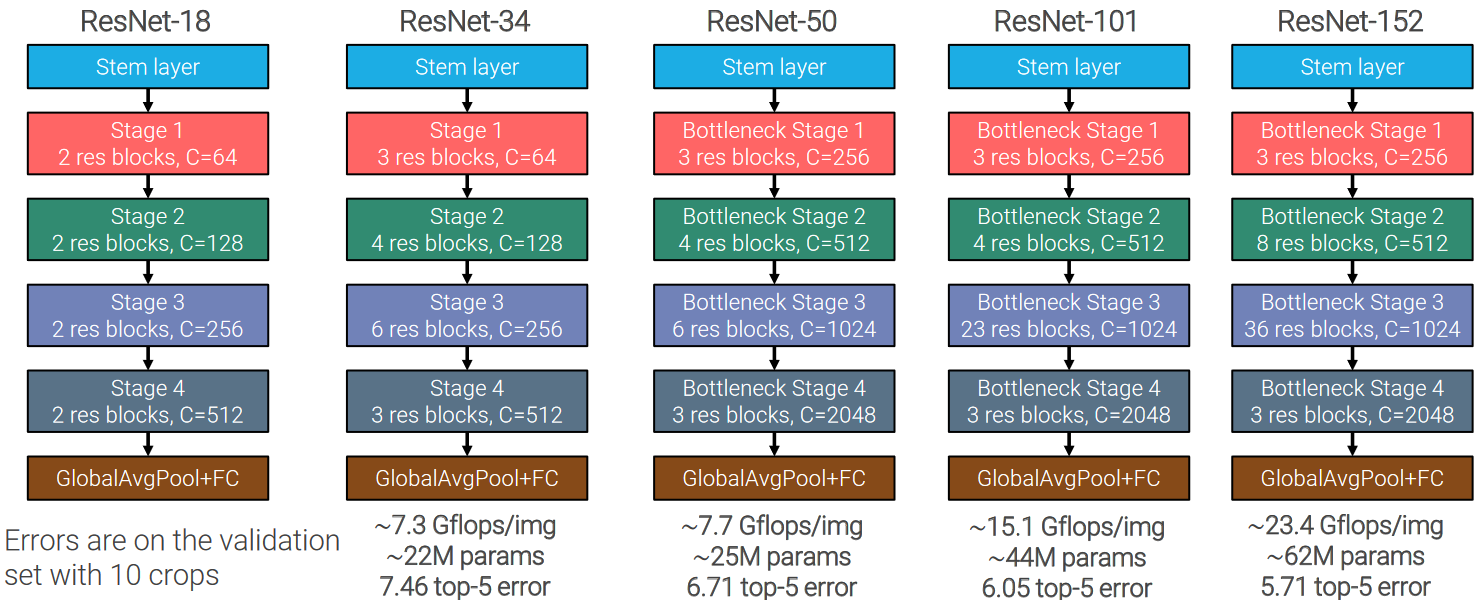
\includegraphics[width=0.8\linewidth]{./img/resnet_variants.png}
%     \caption{ResNet variants. ResNet-18 and ResNet-34 use standard residual blocks. ResNet-50, ResNet-101 and ResNet-152 use bottleneck blocks.}
% \end{figure}

\begin{remark}
    Residual connection creates a smother loss surface.
    \begin{figure}[H]
        \centering
        \begin{subfigure}{0.3\linewidth}
            \centering
            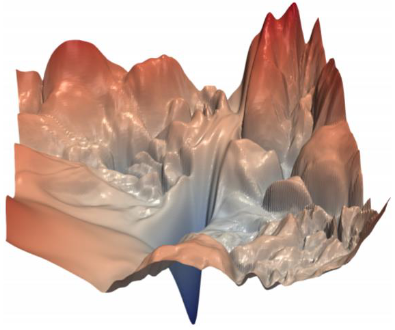
\includegraphics[width=0.7\linewidth]{./img/resnet_loss1.png}        
            \caption{Without skip connections}
        \end{subfigure}
        \begin{subfigure}{0.3\linewidth}
            \centering
            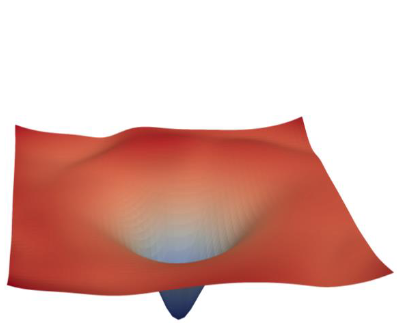
\includegraphics[width=0.7\linewidth]{./img/resnet_loss2.png}        
            \caption{With skip connections}
        \end{subfigure}
        \caption{Loss surface visualized through dimensionality reduction}
    \end{figure}
\end{remark}

\begin{remark}[ResNet as ensemble]
    Skip connections can be seen as a way to create an ensemble-like network as it allows the network to ignore blocks by learning the identity function.
    \begin{figure}[H]
        \centering
        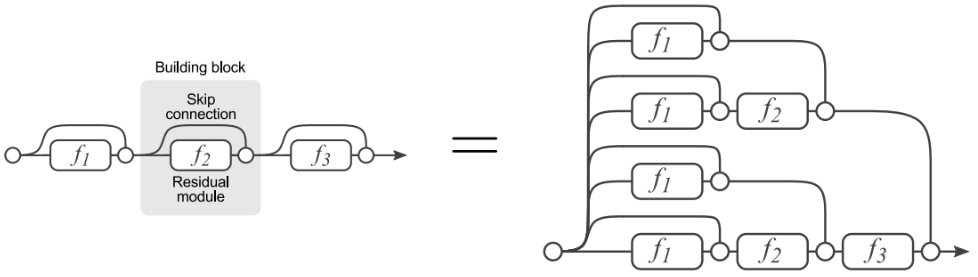
\includegraphics[width=0.6\linewidth]{./img/resnet_ensemble.png}
        \caption{Possible paths of a residual network with three blocks}
    \end{figure}

    Studies show that, in ResNet-56, the gradient updates a subset of the blocks at the time. This is due to the fact that:
    \begin{itemize}
        \item The majority of the possible paths have a length of $\sim 30$.
        \item The gradient magnitude is significant at the first layers (i.e. in shorter paths).
    \end{itemize}
    By multiplying the values of the two points above, results show that the total gradient magnitude is significant only up until paths of length $\sim 20$.
    
    \begin{figure}[H]
        \centering
        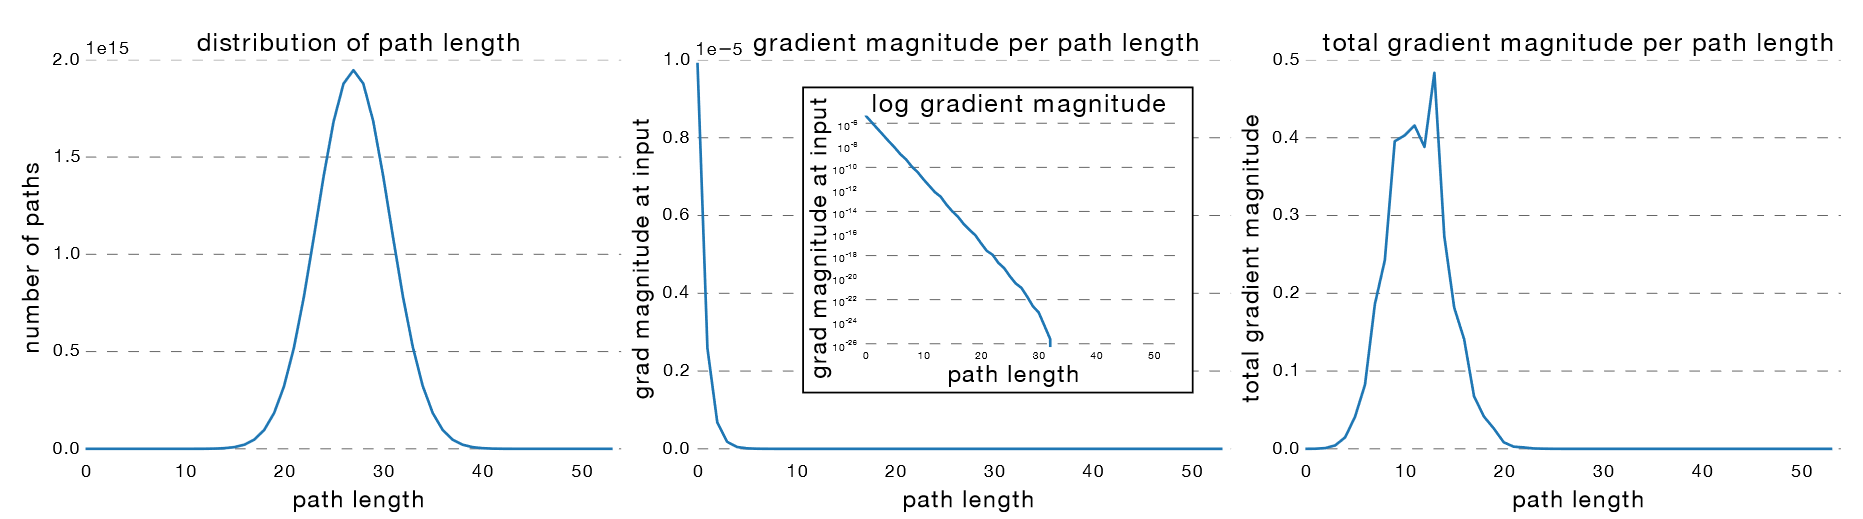
\includegraphics[width=0.95\linewidth]{./img/resnet_ensemble_magnitude.png}
    \end{figure}

    Further experiments show that by randomly deleting layers of the network, the drop in performance, as expected in ensemble models, becomes significant only after a certain number of layers.
    \begin{figure}[H]
        \centering
        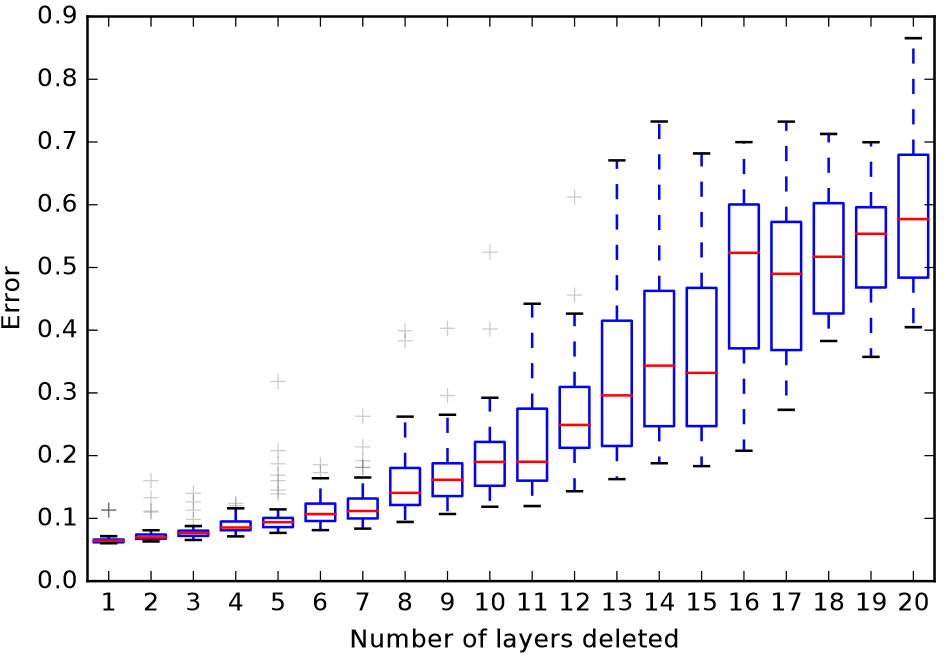
\includegraphics[width=0.4\linewidth]{./img/resnet_ensemble_experiment.png}
    \end{figure}

    Therefore, skip connections do not directly solve the vanishing problem but go around it by creating an ensemble of smaller networks. 
\end{remark}


\subsection{ResNet-v2}

Several improvements over the original ResNet have been made:
\begin{descriptionlist}
    \item[ResNet-B] \marginnote{ResNet-B}
        As the first block of each stage is responsible for halving the spatial dimension, in a bottleneck block this is done by the first $1 \times 1$ convolution. This causes to lose $\frac{3}{4}$ of the input activations as a $1 \times 1$ convolution with stride $\geq 2$ does not have spatial extent. To solve this issue, the halving of the input image is done by the second $3 \times 3$ convolution.

    \item[ResNet-C] \marginnote{ResNet-C}
        The $7 \times 7$ convolution in stem layers is replaced by a sequence of three $3 \times 3$ convolutions, the first one with stride $2$.

    \item[ResNet-D] \marginnote{ResNet-D}
        Similarly to ResNet-B, the $1 \times 1$ convolution used to match the shape of the skip connection has a stride of $2$ and causes a loss of activations. Therefore, stride is dropped and a $2 \times 2$ average pooling with stride $2$ is added before the convolution. 
\end{descriptionlist}

\begin{figure}[H]
    \centering
    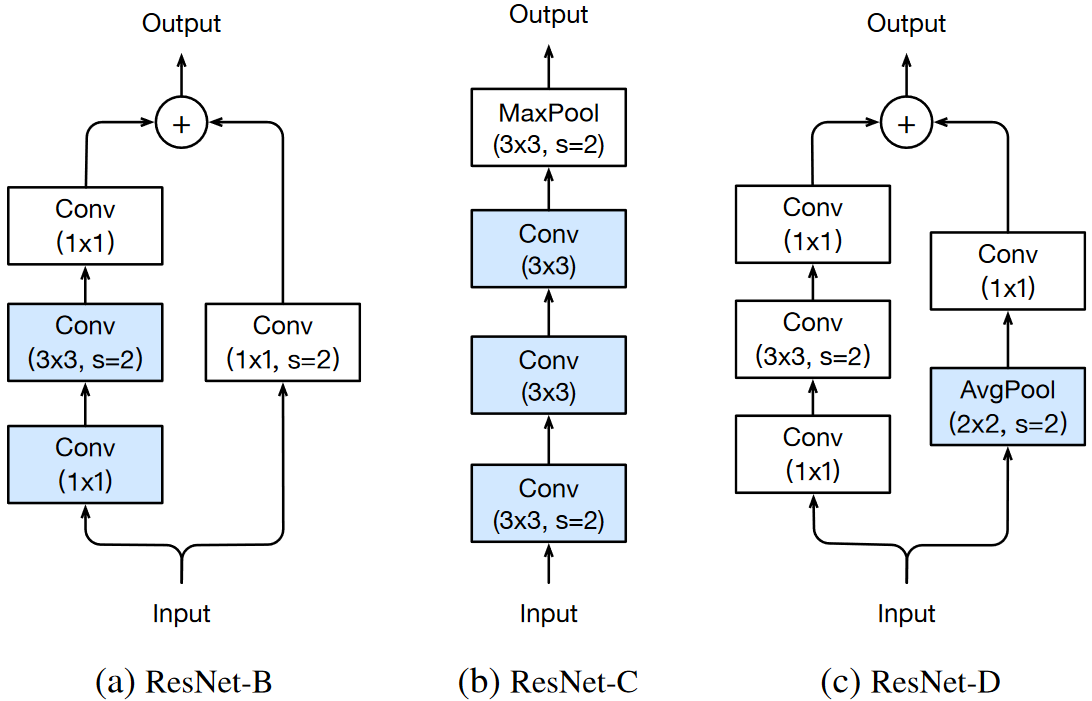
\includegraphics[width=0.5\linewidth]{./img/resnet_v2.png}
\end{figure}


\subsection{Inception-ResNet-v4}

Network with bottleneck-block-inspired inception modules.

\begin{descriptionlist}
    \item[Inception-ResNet-A] \marginnote{Inception-ResNet-A}
        Three $1 \times 1$ convolutions are used to compress the input channels. Each of them leads to a different path:
        \begin{itemize}
            \item Directly to the final concatenation.
            \item To a $3 \times 3$ convolution.
            \item To two $3 \times 3$ convolutions (i.e. a factorized $5 \times 5$ convolution). 
        \end{itemize}
        The final concatenation is passed through a $1 \times 1$ convolution to match the skip connection shape.

    \item[Inception-ResNet-B] \marginnote{Inception-ResNet-B}
        Three $1 \times 1$ convolutions are used to compress the input channels. Each of them leads to:
        \begin{itemize}
            \item Directly to the final concatenation.
            \item A $1 \times 7$ and $7 \times 1$ convolutions (i.e. a factorized $7 \times 7$ convolution). 
        \end{itemize}
        The final concatenation is passed through a $1 \times 1$ convolution to match the skip connection shape.
\end{descriptionlist}

\begin{figure}[H]
    \centering
    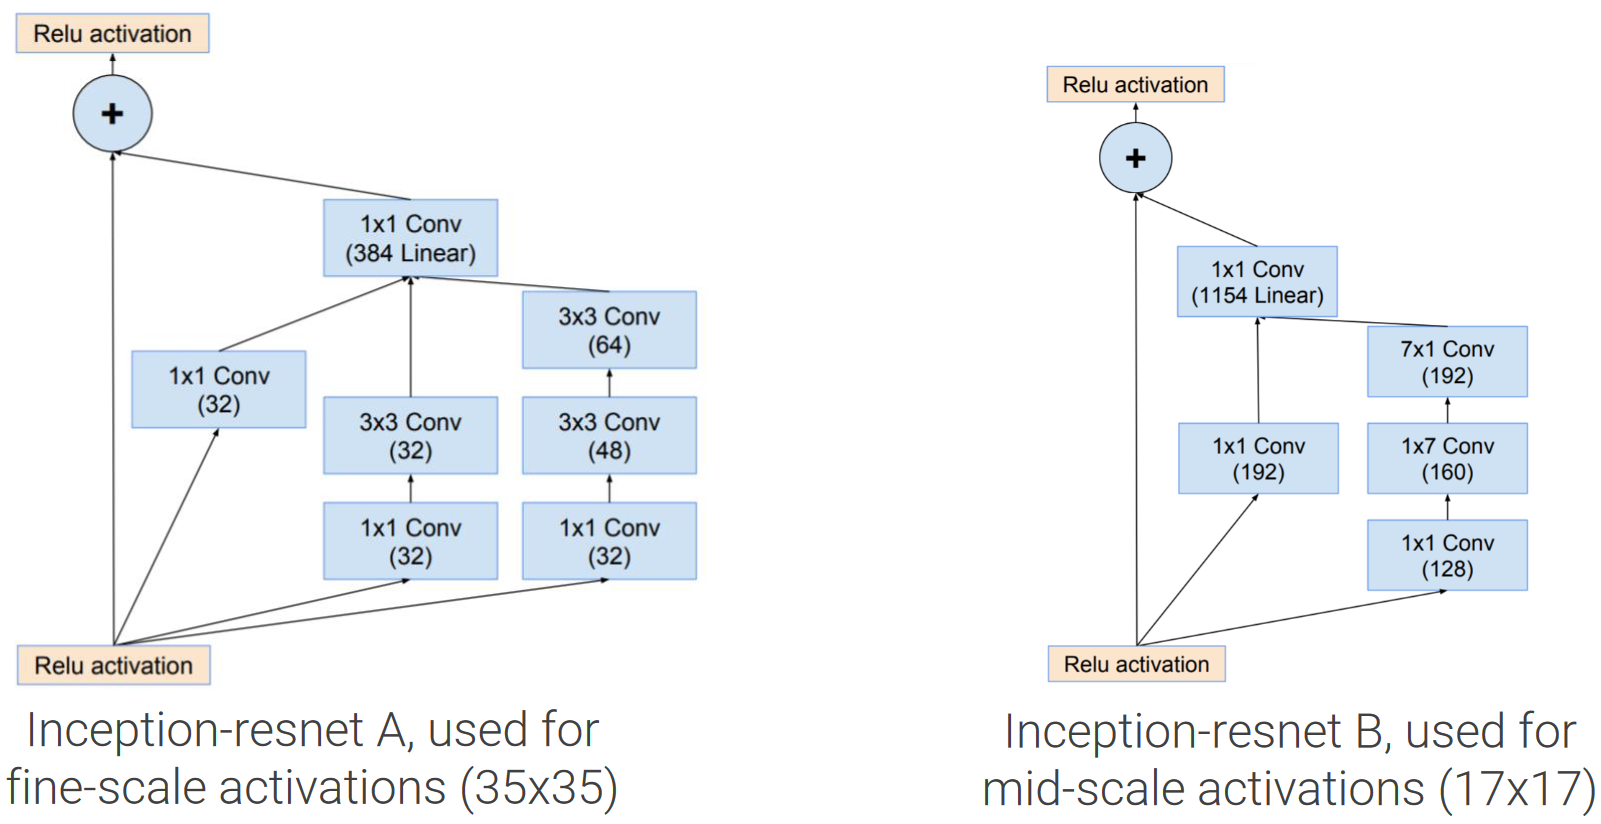
\includegraphics[width=0.65\linewidth]{./img/inception_resnet.png}
\end{figure}



\section{Transfer learning}
\marginnote{Transfer learning}

Adapt a pre-trained network on a new dataset. There are mainly two approaches:
\begin{description}
    \item[Frozen CNN]
        The weights of the pre-trained CNN are kept frozen and a new trainable classification head is added at the end of the model. In this case, the pre-trained model only acts as a feature extractor.

    \item[Fine-tuning] 
        After transferring using the frozen CNN approach, the pre-trained model can be unfrozen (entirely or only the higher layers) and further trained together with the new classification head, usually for a few steps.
\end{description}